\documentclass[draft,final]{vutinfth} % Remove option 'final' to obtain debug information.

% Load packages to allow in- and output of non-ASCII characters.
\usepackage{lmodern}        % Use an extension of the original Computer Modern font to minimize the use of bitmapped letters.
\usepackage[T1]{fontenc}    % Determines font encoding of the output. Font packages have to be included before this line.
\usepackage[utf8]{inputenc} % Determines encoding of the input. All input files have to use UTF8 encoding.

% Extended LaTeX functionality is enables by including packages with \usepackage{...}.
\usepackage{amsmath}    % Extended typesetting of mathematical expression.
\usepackage{amssymb}    % Provides a multitude of mathematical symbols.
\usepackage{amsthm}     % theorems
\usepackage{mathtools}  % Further extensions of mathematical typesetting.
\usepackage{microtype}  % Small-scale typographic enhancements.
\usepackage[inline]{enumitem} % User control over the layout of lists (itemize, enumerate, description).
\usepackage{csquotes}   % Display quotations.
\usepackage{multirow}   % Allows table elements to span several rows.
\usepackage{booktabs}   % Improves the typesettings of tables.
\usepackage{subcaption} % Allows the use of subfigures and enables their referencing.
\usepackage[boxed,algochapter,noend]{algorithm2e} % Enables the writing of pseudo code.
\usepackage[usenames,dvipsnames,table]{xcolor} % Allows the definition and use of colors. This package has to be included before tikz.
\usepackage{pgfplots}
\usepackage{nag}       % Issues warnings when best practices in writing LaTeX documents are violated.
\usepackage{todonotes} % Provides tooltip-like todo notes.
\usepackage[style=alphabetic,maxbibnames=99]{biblatex}  % More control over bibliography
\usepackage{hyperref}  % Enables cross linking in the electronic document version. This package has to be included second to last.
\usepackage[acronym,toc]{glossaries} % Enables the generation of glossaries and lists fo acronyms. This package has to be included last.

\usepackage{standalone} % Allows including standalone content

\addbibresource{bsc_thesis.bib}
\AtEveryBibitem{\clearfield{language}} % don't print language of citation

% recommendation by https://www.overleaf.com/learn/latex/pgfplots_package
\pgfplotsset{width=12cm,compat=1.9}


\pgfplotsset{every picture/.style={line width=0.75pt}} %set default line width to 0.75pt    
% \pgfplotsset{every picture/.style={line width=0.95pt}}

%\usepgfplotslibrary{external} % does not seem to work in Overleaf?!
%\tikzexternalize

% CUSTOM DEFINITIONS
\newtheorem{theorem}{Theorem}
\newtheorem{conjecture}{Conjecture}
\newtheorem{definition}{Definition}
\newtheorem{problem}{Problem}

% macros for commonly used symbols/definitions
\newcommand{\R}{\mathbb R} % real numbers
\newcommand{\Spines}{S} % spine nodes of lobster
\newcommand{\Branches}{B} % branch nodes of lobster
\newcommand{\Leaves}{L} % leaf nodes of lobster
\newcommand{\Emb}{\mathcal E} % embeddings of graphs
\newcommand{\coord}{\gamma} % plane coordinate
\newcommand{\order}{\leq_G} % embeddings of graphs
\newcommand{\probinst}{\pi} % problem instances
\newcommand{\signature}{\varsigma} % dp: partial problem signatures
\newcommand{\depth}{\delta} % depth of partial problem instance

% Define convenience functions to use the author name and the thesis title in the PDF document properties.
\newcommand{\authorname}{Peter Neubauer} % The author name without titles.
\newcommand{\thesistitle}{Practical Examination of Unit Disk Contact Representations} % The title of the thesis. The English version should be used, if it exists.

% Set PDF document properties
\hypersetup{
    pdfpagelayout   = TwoPageRight,           % How the document is shown in PDF viewers (optional).
    linkbordercolor = {Melon},                % The color of the borders of boxes around crosslinks (optional).
    pdfauthor       = {\authorname},          % The author's name in the document properties (optional).
    pdftitle        = {\thesistitle},         % The document's title in the document properties (optional).
    pdfsubject      = {Subject},              % The document's subject in the document properties (optional).
    pdfkeywords     = {a, list, of, keywords} % The document's keywords in the document properties (optional).
}

\setpnumwidth{2.5em}        % Avoid overfull hboxes in the table of contents (see memoir manual).
\setsecnumdepth{subsection} % Enumerate subsections.

\nonzeroparskip             % Create space between paragraphs (optional).
\setlength{\parindent}{0pt} % Remove paragraph identation (optional).

\makeindex      % Use an optional index.
\makeglossaries % Use an optional glossary.
%\glstocfalse   % Remove the glossaries from the table of contents.

% Set persons with 4 arguments:
%  {title before name}{name}{title after name}{gender}
%  where both titles are optional (i.e. can be given as empty brackets {}).
\setauthor{}{\authorname}{}{male}
\setadvisor{Univ.Prof. Dipl.-Inform. Dr.rer.nat.}{Martin Nöllenburg}{}{male}

% For bachelor and master theses:
\setfirstassistant{Dipl.-Ing. B.A.}{Soeren Terziadis}{}{male}
%\setsecondassistant{Pretitle}{Forename Surname}{Posttitle}{male}

% Required data.
\setregnumber{00725263}
\setdate{01}{10}{2022} % Set date with 3 arguments: {day}{month}{year}.
\settitle{\thesistitle}{\thesistitle} % Sets English and German version of the title (both can be English or German). If your title contains commas, enclose it with additional curvy brackets (i.e., {{your title}}) or define it as a macro as done with \thesistitle.
%\setsubtitle{Optional Subtitle of the Thesis}{Optionaler Untertitel der Arbeit} % Sets English and German version of the subtitle (both can be English or German).

\setthesis{bachelor}
\setcurriculum{Software \& Information Engineering}{Software \& Information Engineering}

\includeonly{1_introduction, 2_preliminaries,3_related-work,4_dynamic-program,5_heuristic,6_evaluation,7_conclusion}

%%%%%%%%%%%%%%%%%%%%%%%%%%%%%%%% COMMENTS FUNCTION %%%%%%%%%%%%%%%%%%%%%%%%%%%%%%%%
\usepackage{todonotes}
\newcommand{\personaltodo}[4][noinline]{\todo[#1,color=#2]{#3: #4}}
\newcommand{\peter}[2][noinline]{\personaltodo[#1]{gray!30}{PN}{#2}}
\newcommand{\soeren}[2][noinline]{\personaltodo[#1]{teal!30}{ST}{#2}}
\newcommand{\martin}[2][noinline]{\personaltodo[#1]{blue!30}{MN}{#2}}
%%%%%%%%%%%%%%%%%%%%%%%%%%%%%%%% COMMENTS FUNCTION %%%%%%%%%%%%%%%%%%%%%%%%%%%%%%%%

\begin{document}

\frontmatter % Switches to roman numbering.
% The structure of the thesis has to conform to the guidelines at
%  https://informatics.tuwien.ac.at/study-services

%\addtitlepage{naustrian} % German title page (not for dissertations at the PhD School).
\addtitlepage{english} % English title page.
\addstatementpage

%\begin{danksagung*}
%\todo{Ihr Text hier.}
%\end{danksagung*}

%\begin{acknowledgements*}
%\todo{Enter your text here.}
%\end{acknowledgements*}

%\begin{kurzfassung}
%\todo{Ihr Text hier.}
%\end{kurzfassung}

\peter[inline]{inline comment}
\soeren[inline]{inline comment}
\martin[inline]{inline comment}
\peter{side comment}
\soeren{side comment}
\martin{side comment}
\begin{abstract}
Disk contact graphs are graphs which can be drawn in the plane such that every disk represents a vertex, and disk contact represents graph edges. These graphs and their variants form are a lively research topic in the field of Algorithmic Geometry. This work focuses on recognition problems of unit disk contact on restricted graph classes, specifically caterpillars and lobsters. These restricted classes are easier to recognize than general planar graphs or even trees, with some caveats.

We formally review the related problems, their complexity, limitations and hypotheses. Then we formulate two algorithms to decide, in particular, whether a given lobster admits an x-monotone weak unit disk contact representation on a triangular coordinate grid. One is a dynamic programming algorithm from the literature with some performance modifications, which decides the problem exactly. The other is a fast, inexact, greedy heuristic approach.

Both algorithms are implemented in an accompanying software project. We employ this program for experimental analysis of the presented approaches. The examination covers a complete enumeration of all relevant lobsters up to a spine length of $7$ nodes. It regards the run time of both implementations and accuracy of the heuristic, showing that the heuristic algorithm is up to $100\times$ faster and, though generally less reliable on larger instances, correctly decides about $70\%$ of yes-instances with spine length $7$.
\soeren[inline]{I don't completely recall, but I think this was still Work in Progress right? Can (and should) definitely be expanded}
\peter[inline]{Expanded and ready for next review.}
\end{abstract}

% Select the language of the thesis, e.g., english or naustrian.
\selectlanguage{english}

% Add a table of contents (toc).
\tableofcontents % Starred version, i.e., \tableofcontents*, removes the self-entry.

% Switch to arabic numbering and start the enumeration of chapters in the table of content.
\mainmatter


\chapter{Introduction}

A disk contact graph is a graph for which there exists a mapping of all vertices to disks on the plane such that, if two vertices are connected, their respective disks are in contact with each other.
Since the formulation of the circle packing theorem~\cite{Koebe1936}, we know that every planar graph is a disk contact graph.

Various practical applications, such as wireless communication towers~\cite{Hale1980}, require us to consider the restricted case of \emph{unit disk graphs} (also known as \emph{coin graphs}), in which all disks in the graph's planar embedding are of one unit size.

Not every planar graph is a unit disk contact graph. Naturally, we have to consider the associated recognition problem: given a planar graph $G$, does it admit an embedding in the plane using unit disks? 
This problem is NP-hard~\cite{Breu1998}. The same complexity persists even restricting the problem only to trees, as shown by Bowen et al.~\cite{Bowen2015}.

\begin{figure}
    \centering
    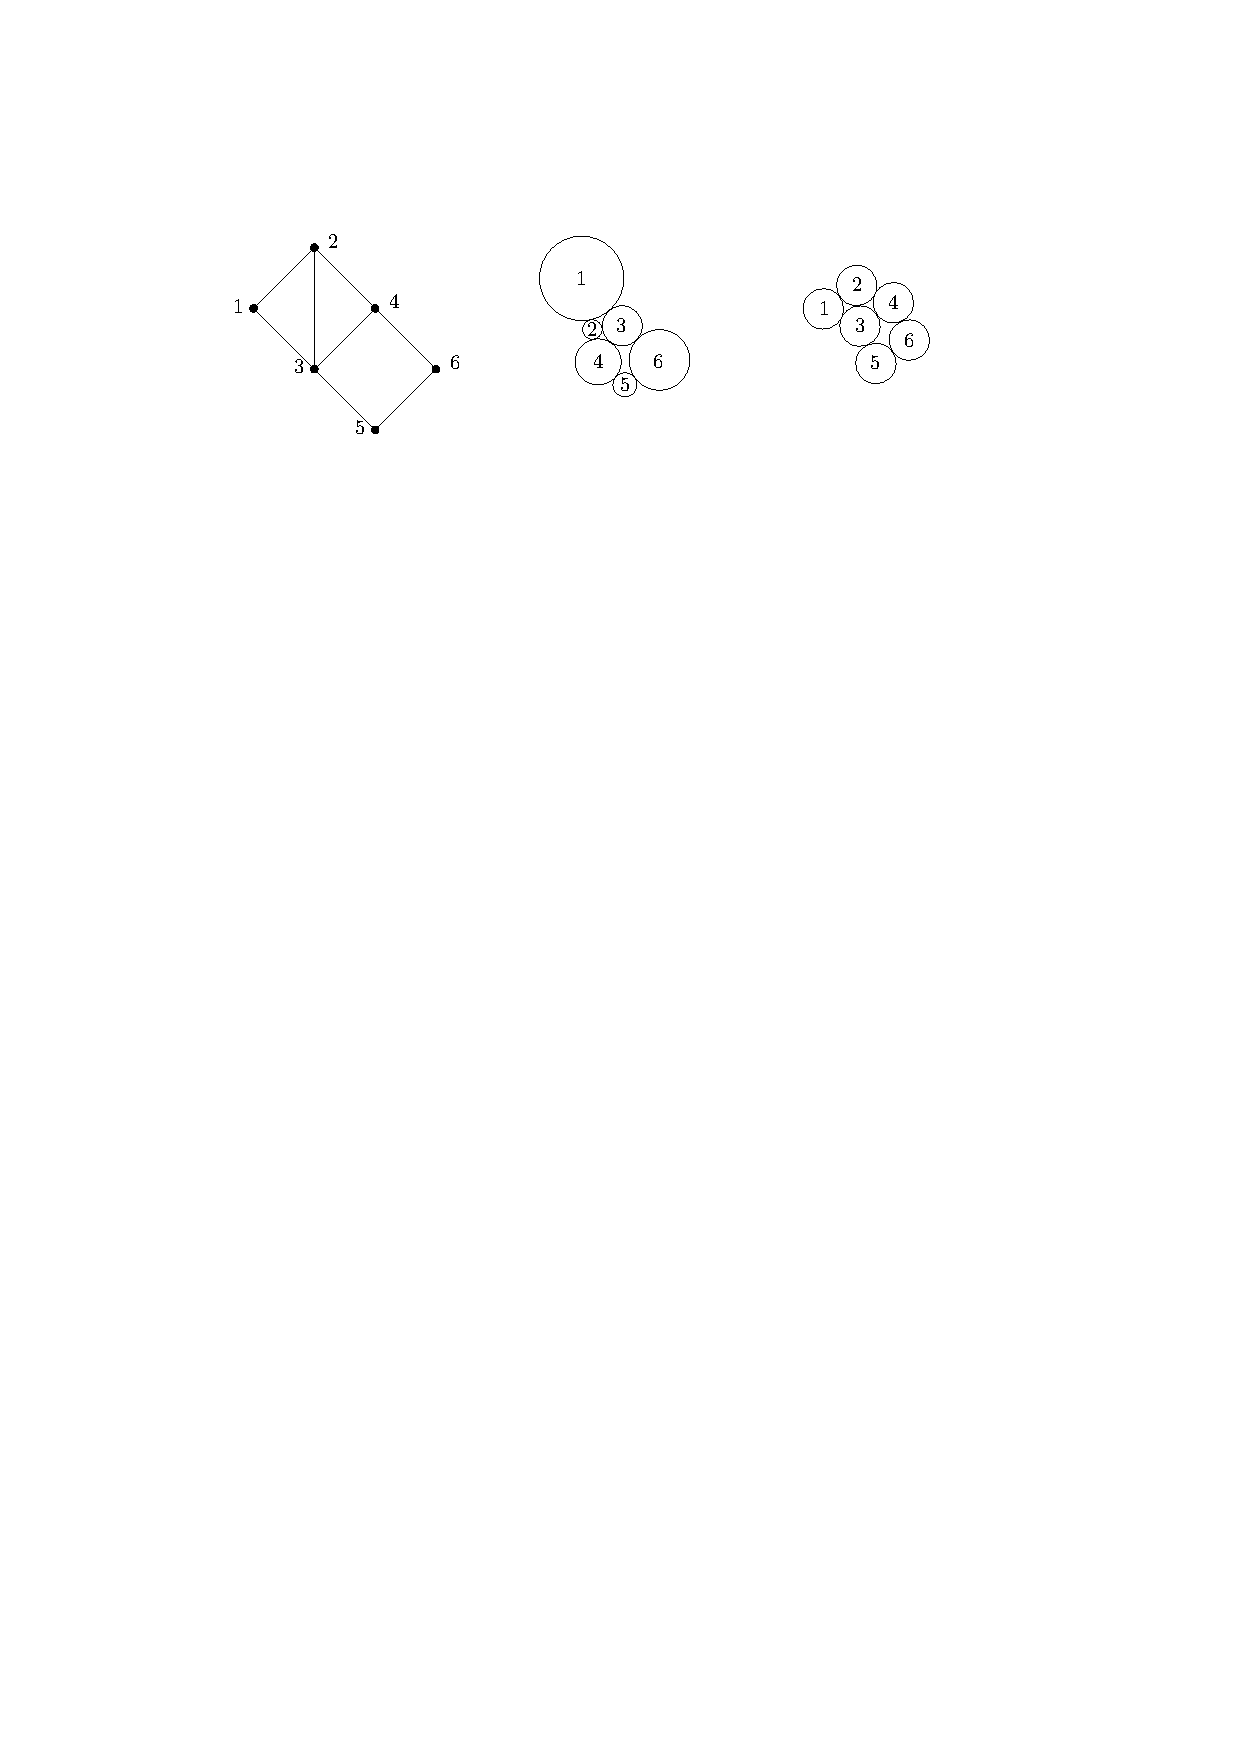
\includegraphics{graphics/ch1_introduction.pdf}
    \caption{Different representations of the same graph.}
    \label{fig:ch1_introduction}
\end{figure}

If even trees are too complex to decide in polynomial time, then where is the line of tractability? Coming at the problem from the other direction, we can identify graphs for which this problem is definitely in P.

A caterpillar is a tree which consists only of a string of connected vertices called a ``spine'' or ``backbone'', and an arbitrary number of leaf nodes connected to the spine.
It is possible to decide the problem for caterpillars in linear time~\cite{Klemz2015}~\cite{Cleve2020}. Klemz et al. show this result under the ``proper'' or ``strict'' mode of disk contact, where the interior-disjoint disks are in contact if and only if there is an edge between their nodes. Cleve uses the slightly modified notion of ``weak'' disk contact, in which the corresponding disks may touch even between unconnected vertices.

We conclude that the line between graph classes for which the recognition problem is tractable and those for which it remains intractable lies somewhere between caterpillars and trees. Perhaps there is some pertinent quality about them that determines the problem's complexity.

This thesis is concerned with the complexity of the recognition problem on the lobster, one such in-between class. Our approach uses the ``weak'' disk contact notion.

A lobster is a tree which, similar to the caterpillar, has a connected vertex string for a spine.
The spine vertices may further be connected to subtrees with a depth of at most two, i.e. ``expanding'' the caterpillar concept by one step from the leaves.

Our main question is whether the lobster, like the caterpillar, can be recognized in linear time. We also aim to provide a practical method of constructing a unit disk contact embedding for a given instance. Additionally, we are curious to know how fast and how accurate our solution is.

It is conjectured that lobsters are x-monotone, i.e. that any unit disk contact lobster can be embedded without any ``u-turns'' in the spine~\cite{Bhore2021}. With the \texttt{udcrgen} software developed in conjunction with this thesis, we provide a tool which can empirically evaluate such x-monotone lobsters through exhaustive enumeration and testing of small lobsters.

If lobsters are indeed x-monotone, and another assumption on the alignment of the embedding on a triangular grid also holds, it follows that the dynamic program implemented by \texttt{udcrgen} decides the problem in linear time~\cite{Bhore2021}. Beyond the asymptotic time constraints given by theory, our implementation should use prudent shortcuts and methods to achieve good performance in practice.

Furthermore, we present a heuristic to embed lobsters. Both approaches run in linear time, but the dynamic program requires us to consider an impractically large set of partial solutions. We examine both approaches with regards to correctness and run time.

The results thus presented narrow a gap in our understanding of the complexities of the unit disk contact problem. They offer tools for solving lobsters in particular, and a step towards further research.

In Chapter~2, we introduce all necessary terminology and formal definitions, building up to the embedding problems which we approach in the later chapters.
Chapter~3 delves into the literature which forms the basis of this work and other interesting related works.
Chapter~4 explains our reliable approach for deciding the UDCR problem for any given lobster in linear time. It covers theoretical and implementation aspects.
Chapter~5 explains our faster, but not always correct, approach to the same problem.
Chapter~6 describes our empirical evaluation of the two approaches. Using the implementation written in conjunction with this thesis, we exhaustively cover lobsters up to spine length 7. We compare our algorithms with regards to run time and correctness.
In Chapter~7, we summarize the results and consider open questions for future work.



\chapter{Preliminaries}

\soeren[inline]{in general I think you can reduce the number of Definition environments drastically. Graph, embedding, planar graph and many more can be defined in simple Text. I know that this seems unintuitive, a clear cut definition being more precise. There is room for this, If you introduce something which is both uncommon or very specific and important to your work (like the concept of a unit disk contact representation). Definitions in text read easier AND the definition environment itself is elevated as the core important concept a reader should understand.}\peter[inline]{should be better now}

Starting from the basics, this chapter introduces the definitions and notation used in this work.

\section{Graph Classes}

A graph $G = (V, E)$ is defined by its vertices $V = \{ v_0, \ldots , v_n \}$ and edges $E \subseteq \{ v, w \}, v, w \in V$. Though all our graphs are undirected, we use the edge notation $(v, w)$ for readability without implying a direction.

A \emph{drawing} of a graph is a representation of the vertices and edges of $G$ in the plane. A drawing contains an implied mapping of a planar coordinate to every graph vertex, and of a curve to every edge such that the endpoints of the curve are the planar coordinates of the incident vertices.

A graph $G$ is \emph{planar} if there exists a drawing of $G$ such that none of the curves, which represent the edges, intersect or overlap. Such is always the case for \emph{trees}.

A \emph{spined graph} is a tree $G = (\Spines \cup \mathcal T, E)$, where $\Spines = \{ s_1, \ldots, s_k \}$ is the set of \emph{spine vertices} and $\mathcal T$ are the \emph{subtree} vertices. The spine is a connected string: $(s_i, s_{i+1}) \in E$. The depth $d$ of $G$ is defined as the maximum path distance from any $t \in \mathcal T$ to any spine in $\Spines$.
\soeren{Again pull depth out of the definition. One thing per definition.}\peter{spined graph is no longer in a def env. good?}

\begin{figure}
    \centering
    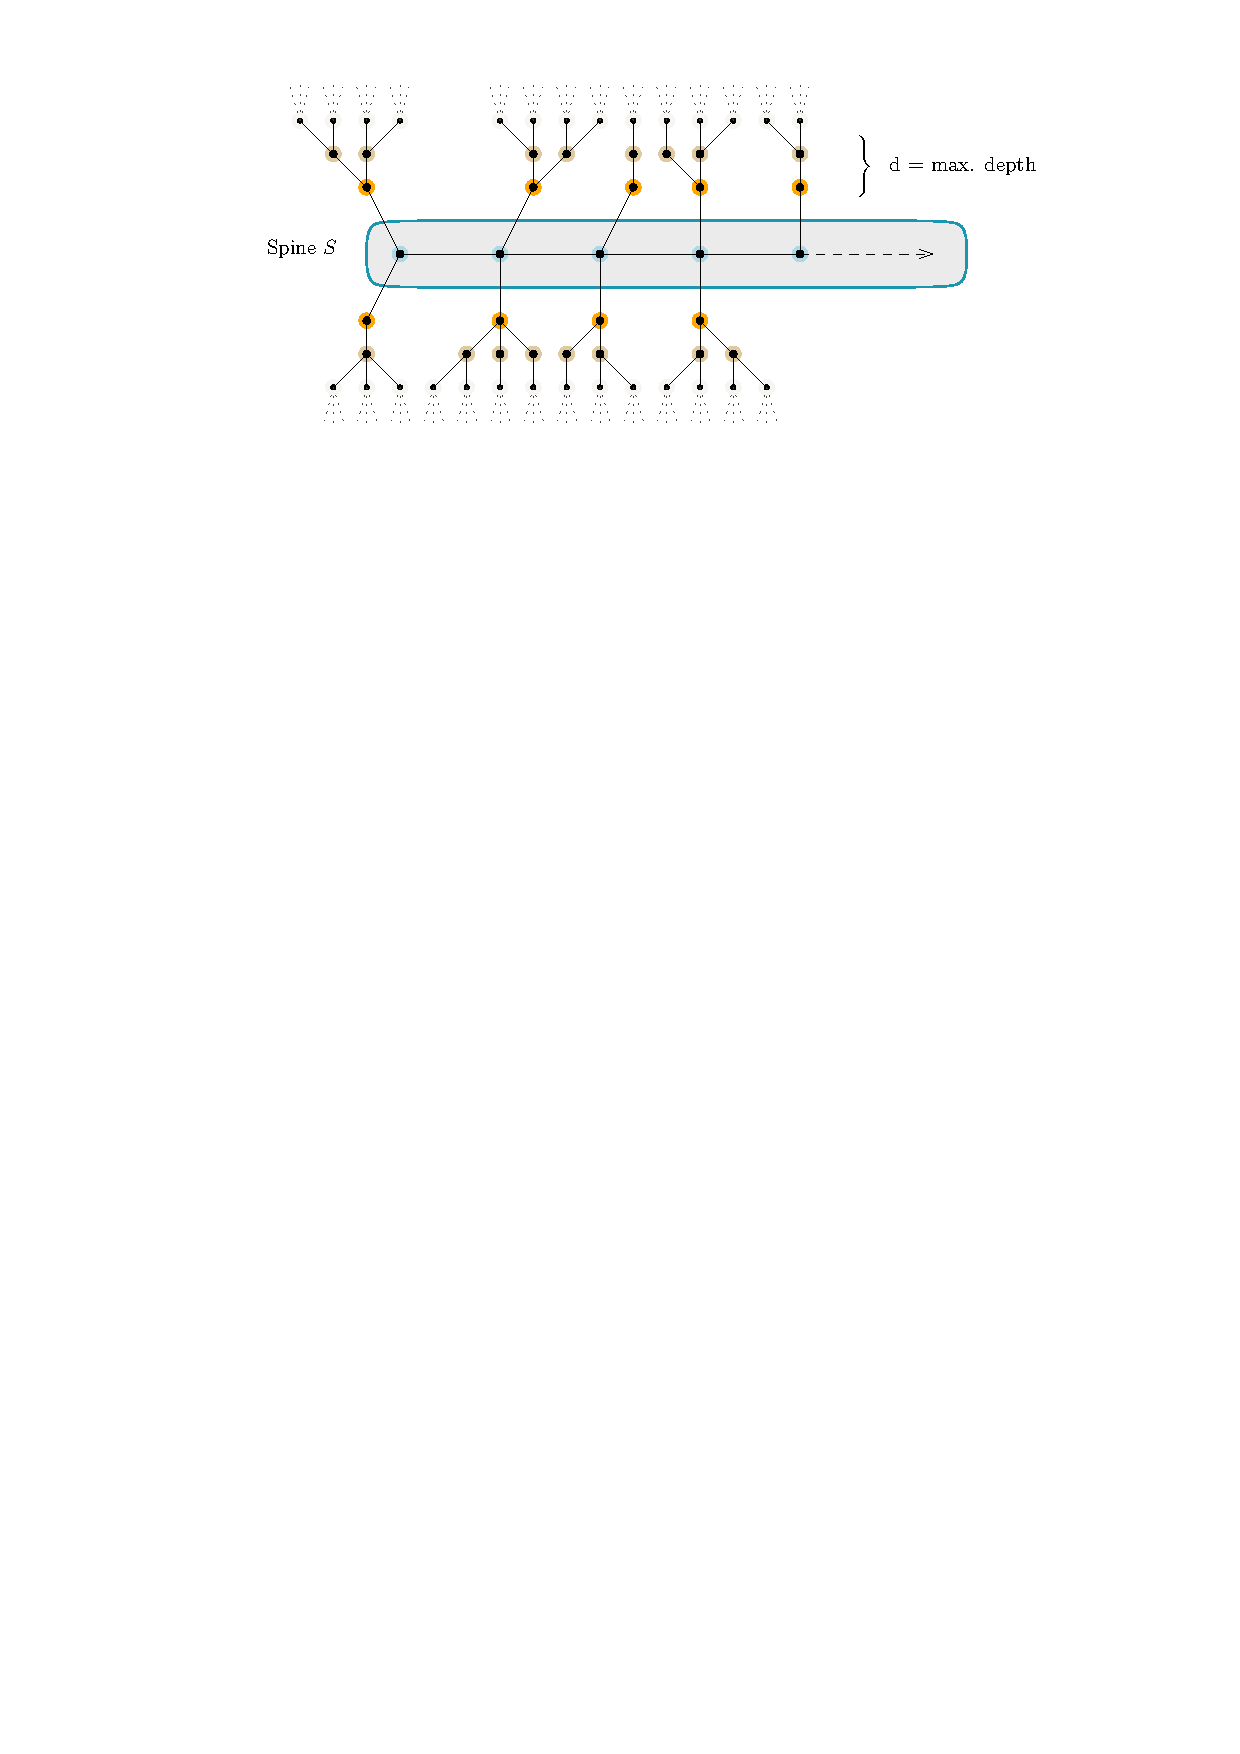
\includegraphics{graphics/ch2_spinedgraph.pdf}
    \caption{A spined graph consists of a string of vertices identified as the \emph{spine}, here marked in blue. Connected to the spine vertices, we find the subtrees rooted in the orange vertices. With unbounded depth and unbounded spine length, spined graphs are little more than trees. However, by bounding $d$ by a constant, we treat ourselves to a new class of graph, simpler than the general tree.}
    \label{fig:ch2_spinedgraph}
\end{figure}

A \emph{caterpillar} is a spined graph $(\Spines \cup \Leaves, E)$ with depth $d=1$, where $\Leaves$ is the set of \emph{leaves}. $\Spines$ and $\Leaves$ are disjoint sets. Every leaf $l \in \Leaves$ is connected to its parent spine vertex $p(l) \in \Spines$: $(l, p(l)) \in E$.

We are now prepared to introduce the graph class which is the core subject of our examination.

\begin{definition}[Lobster]
A lobster is a spined graph $(\Spines \cup \Branches \cup \Leaves, E)$ with depth $d=2$, where $\Branches$ is the set of \emph{branches} and $\Leaves$ is the set of \emph{leaves}.  $\Spines$, $\Branches$ and $\Leaves$ are mutually disjoint sets.

Every branch $b \in \Branches$ is connected to its parent spine vertex $p(b) \in \Spines$: $(b, p(b)) \in E$. Every leaf $l \in \Leaves$ is connected to its parent branch $p(l) \in \Branches$: $(l, p(l)) \in E$.
\end{definition}

\begin{figure}
    \centering
    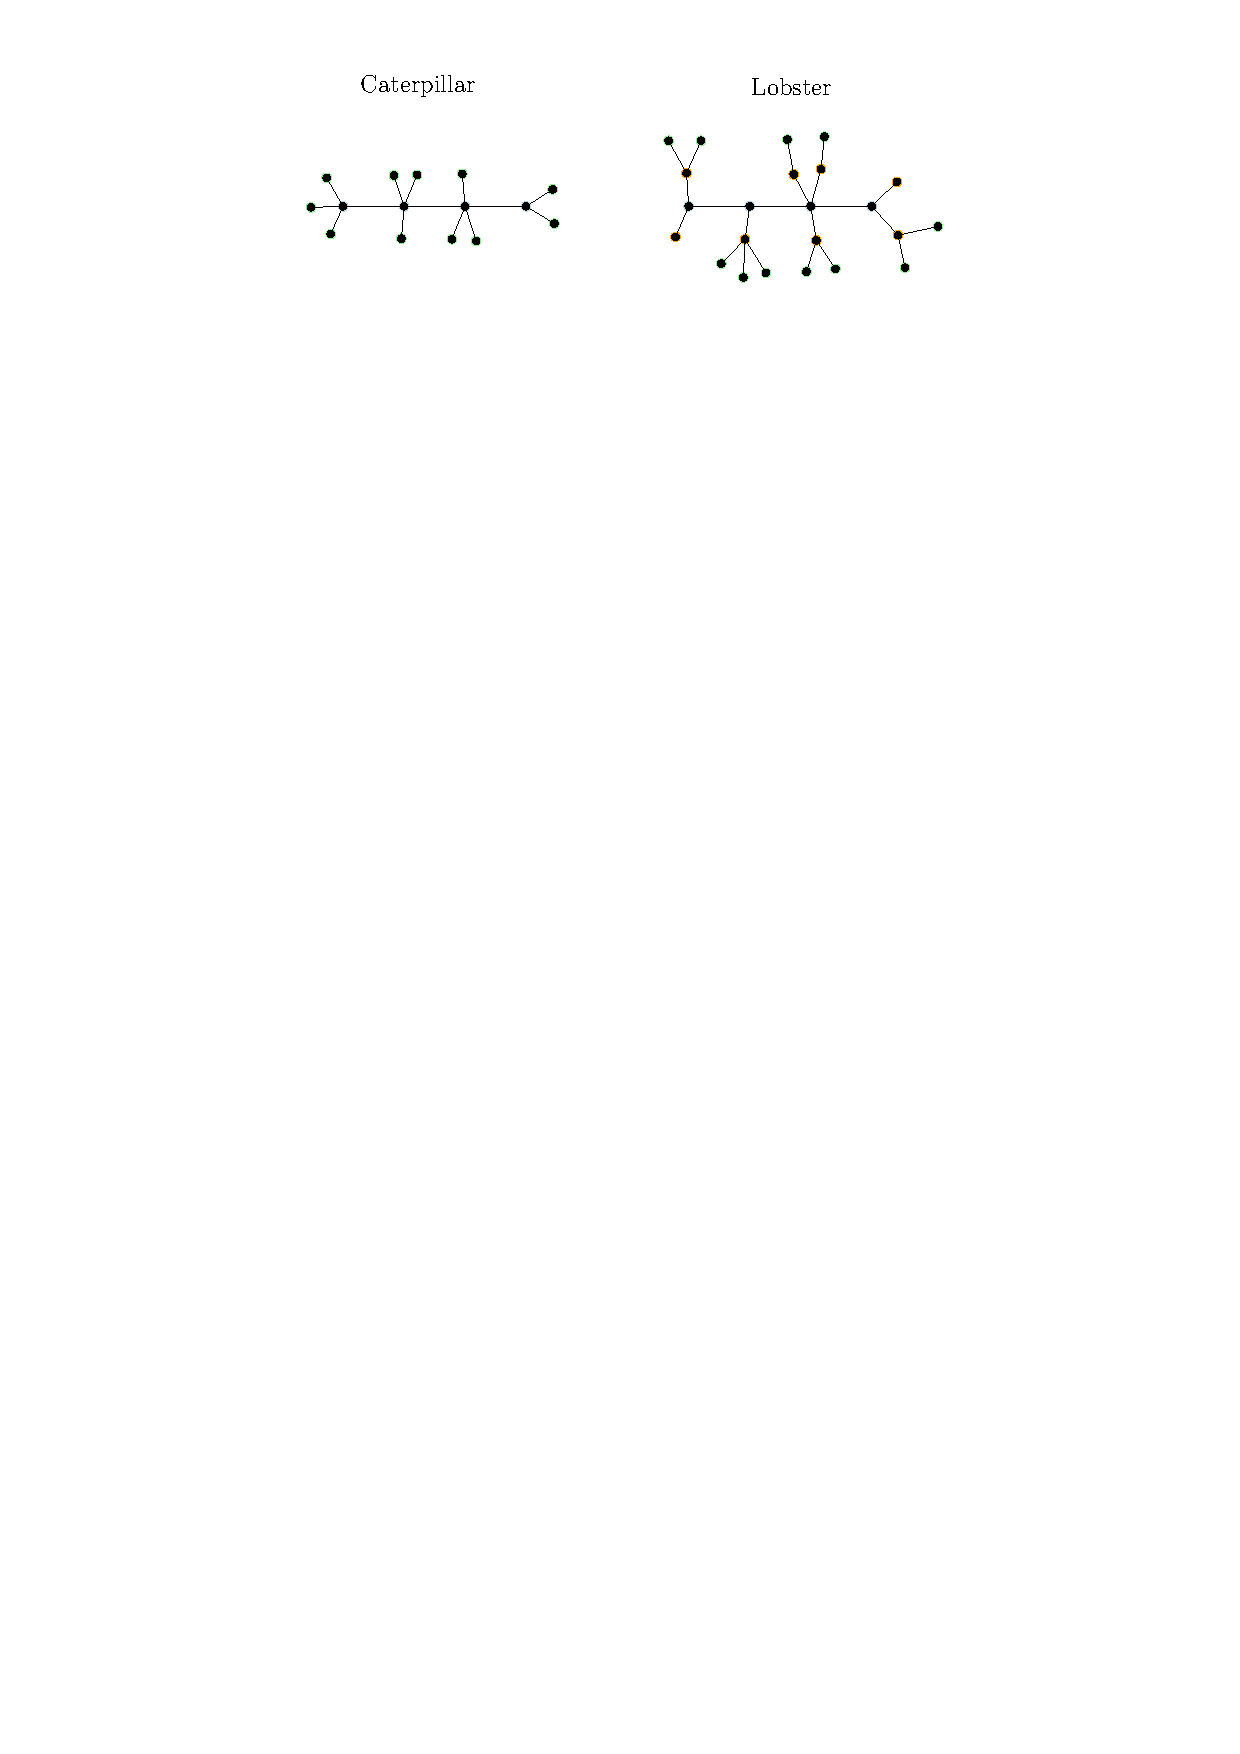
\includegraphics{graphics/ch2_caterpillar_lobster.pdf}
    \caption{The caterpillar and lobster, shown here, are the only kinds of spined graphs which we explore in this thesis.}
    \label{fig:ch2_caterpillar_lobster}
\end{figure}

\section{Representations}

A \emph{combinatorial embedding} (or just \emph{embedding}) of a graph in the plane encodes the topological properties of the graph. For each vertex, the embedding defines the clockwise-ordered permutation of its neighbors. The embedding is independent of any specific planar coordinates for vertices and edges, but every drawing of a planar graph induces an embedding.

In this thesis, we define the \emph{embedding function} $d$ over $G$ as a bijection $d: V \mapsto \R^2$, which maps vertices to coordinates in the plane. In the common node-link diagram representation, we would draw straight lines to represent the edges. The notation $d$ is short for ``disk'' due to the graph representations below for which we use it.

\soeren[inline]{You define Embedding. Maybe it is helpful to define drawing as the mapping of vertices and edges into the plane and then define the concept of a combinatorial embedding, uniquely defined by such a drawing. Then you can say that in contrast to the usual definition of a drawing, you want to represent graphs differently as unit disk representations, but you have the concept of an embedding, and you can say that a unit disk representation \emph{induces} an embedding by using the centerpoint straight line connections to obtain a drawing and the embedding of that drawing, is also the embedding of the unit disk representation.}
\peter[inline]{I defined it somewhat, but suspect that it needs additional review.}

The \emph{Euclidean norm} $||v||, v = (v_x, v_y)$, is the straight-line length of the vector $v$. $||v|| = \sqrt{v_x^2 + v_y^2}$. $||v_1 - v_2||$ is the distance between the points $v_1$ and $v_2$.

The most common notions of graph drawings represent vertices as points. Numerous alternative representations exist. Drawings in which vertices are represented as disks are of particular interest to us.

\begin{definition}[Disk Contact Representation]
\label{def:ch2_DCR}
Let $G = (V, E)$ be a graph and $d$ be an embedding function over $G$. Further let $w: V \mapsto \mathbb R$ be a \emph{weight function} for the vertices of $G$ such that

\begin{align*}
\lVert d(v_1) - d(v_2) \rVert &= \frac12(w(v_1) + w(v_2)) &\text{ if } (v_1, v_2) \in E \text{ and} \\ \lVert d(v_1) - d(v_2) \rVert &> \frac12(w(v_1) + w(v_2)) &\text{ otherwise.}
\end{align*}

Then $D = (d, w)$ constitutes a \emph{disk contact representation} of $G$.
\end{definition}

\begin{definition}[Weak Disk Contact Representation]
\label{def:ch2_WDCR}
Let $G = (V, E)$ be a graph, $d$ be an embedding function over $G$ and $w$ be a weight function for $V$ such that

\begin{align*}
\lVert d(v_1) - d(v_2) \rVert &= \frac12(w(v_1) + w(v_2)) &\text{ if } (v_1, v_2) \in E \text{ and} \\ \lVert d(v_1) - d(v_2) \rVert &\ge \frac12(w(v_1) + w(v_2)) &\text{ otherwise.}
\end{align*}

Then $D = (d, w)$ constitutes a \emph{weak disk contact representation} of $G$.
\end{definition}

When we want to explicitly refer to the contact notion from Definition~\ref{def:ch2_DCR}, in contrast to the ``weak'' contact from Definition~\ref{def:ch2_WDCR}, we call it ``strict'' or ``proper'' contact. In the rest of this thesis, we mainly concern ourselves with weak contact. Thus, the weak contact notion is assumed as the default in every context from now on unless explicitly specified otherwise. Regardless, the further definitions involving disk contact can be used both with weak and strict notions of contact.

$G$ is a \emph{disk contact graph} if it admits a disk contact representation. A disk contact graph can be drawn by drawing for each vertex $v$ a disk centered at $d(v)$ with diameter $w(v)$. The disk of $v$ precisely touches the disks of neighbouring vertices. Under strict contact, it does not touch any other disks. Under the weak contact notion, disks may touch even if there is no edge between them. In a drawing using disks, there are no curves to represent the edges beyond the disks being in contact or not. Note that every strict disk contact graph is also a weak disk contact graph.

\soeren{I would state this before the definition of the weak unit disk graphs and remove unnecessary words. 'The famous circle packing theorem establishes an equivalence between disk contact representations and planar graphs.' Citation should be in the statement. I added it here as an example. Old citation should be removed.}
\peter{Moved before unit disks. Good enough?}

The famous \emph{circle packing theorem}~\cite{Koebe1936} states that every planar graph admits a (strict) disk contact representation.

Let $G = (\Spines \cup \mathcal T, E), \Spines = \{ s_1, \ldots, s_n \}$ be a spined graph and $D$ be a disk contact representation. $D$ is \emph{x-monotone} if $\forall i > 1: d_x(s_{i+1}) > d_x(s_i),$ where $d_x(v)$ is the x-component of the embedded coordinate of $v$. Informally, the spine ``goes from left to right''.

If it holds for the weight function $w$ of a disk contact representation of $G = (V, E)$ that $\forall v\in V: w(v) = 1$, then we call it a \emph{unit disk contact representation}, shortening ``unit disk contact'' to UDC for readability. $G$ is a UDC graph or UDCG.

Let $D = (d, w)$ be a weak disk contact representation in which $d$ maps all vertices to points from the set $\{ (x + \frac y2, \frac{\sqrt3}2 y) \mid x, y \in \mathbb Z \}$. This set describes the intersection points of a \emph{triangular grid} in the plane, and we call $D$ a \emph{tri-grid representation}. Every such grid point $\coord$ has a \emph{neighborhood}
\begin{align*}\Gamma(\coord) = \Bigg\{ &\coord + (-1, 0); \coord + \left(-\frac12, \frac{\sqrt3}2\right); \coord + \left(\frac12, \frac{\sqrt3}2\right);\\
&\coord + (1, 0); \coord + \left(\frac12, -\frac{\sqrt3}2\right); \coord + \left(-\frac12, -\frac{\sqrt3}2\right) \Bigg\}.\end{align*}
The more restricted \emph{x-monotone neighborhood}
\begin{align*}\Gamma^{x+}(\coord) = \left\{ \coord + \left(\frac12, \frac{\sqrt3}2\right); \coord + (1, 0); \coord + \left(\frac12, -\frac{\sqrt3}2\right) \right\}\end{align*}
includes only those neighbors with a larger x-coordinate than $\coord$.

The triangular grid lends itself to UDC representations because the distance between two neighbor coordinates on the triangular grid is exactly $1$. Consequently, unit disks embedded at neighboring tri-grid points are in contact. So, if $G = (V, E)$ is a disk contact graph, $D = (d, w)$ is a UDC representation, $v \in V, \coord = d(v)$ and $(v, u) \in E$, then $d(u) \in \Gamma(\coord)$.

\section{Problems}

A \emph{recognition problem} is a computational problem in which the goal is to find an algorithm which decides, for a given input from a larger domain, whether that input belongs to a certain smaller class or set in the domain. We say that the algorithm \emph{recognizes} the set.

The broadest problem that we are interested in discussing here is, in the following two variants:

\begin{problem}[Strict UDC Recognition]
Given a graph $G$, does $G$ admit a strict UDC representation?
\label{prob:strict-udc}
\end{problem}

\begin{problem}[Weak UDC Recognition]
Given a graph $G$, does $G$ admit a weak UDC representation?
\label{prob:weak-udc}
\end{problem}

These problems are successors to the original disk contact problem, answered by the above mentioned circle packing theorem. Now restricted to unit size disks, solutions to these problems already exist for the restricted graph class of caterpillars~\cite{Klemz2015}~\cite{Cleve2020}, to be reviewed in Chapter~\ref{chp:related-work}.

As promised in the introduction, we now tie into current research by focusing our attention on the subclass of lobsters. Under the current state of knowledge, we have no algorithm to answer these problems in polynomial time. We can however make some concessions in the form of assumptions to pull the problem into our analytic reach~\cite{Bhore2021}.

\begin{problem}[Tri-Grid X-Monotone UDC Recognition for Lobsters]
Given a lobster $G$, does $G$ admit a weak x-monotone UDC representation on the triangular grid?
\label{prob:weak-udc-lobster}
\end{problem}
\soeren[inline]{I would call this the Weak UDCG Recognition Problem for Lobsters. Second I think you can define a problem environment as a normal theorem environmant. This looks slightly out of place. I also think this should be the last thing in the preliminaries, where you first introduce what a recognition problem is, then specify the recognition problem for weak trigrid UDCG (which should be defined as graphs taht admit a weak UDCR on a trigrid) and in particular for lobsters. Only the most specific variant of that should be in the problem environment.}
\peter[inline]{problem is now a theorem. weak is default.}

Unit disks on the triangular grid are packed decently dense. Tighter packing configurations exist, but because this grid is nice and regular and our relevant spine graphs---lobsters---only extend up to two neighbors from the spine, we can assume that the slightly sub-optimal density of our chosen packing configuration does not impact our results compared to the arbitrary configuration. In other words, we assume that a given lobster $G$ admits a tri-grid UDC representation if it admits any UDC representation. This assumption also motivates our use of the weak contact notion, which ``unlocks'' the tri-grid configuration for easier analysis.

Likewise, we allow ourselves the restriction to x-monotone solutions based on the unproven assumption that a given lobster $G$ admits an x-monotone UDC representation if it admits any UDC representation. As there is no combinatorial embedding prescribed for $G$, no branch necessarily has to be above or below the spine. Yet, to refute our x-monotonicity assumption, a counter-example lobster would have to have some configuration of branches and leaves such that all its possible UDC representations enforce either an acute ($60^\circ$) ``bend'' in the spine, or two consecutive obtuse ($120^\circ$) bends in the same direction. By superficial experimentation, it appears that such configurations do not occur.

If our assumptions should hold, then solving Problem~\ref{prob:weak-udc-lobster} is equivalent to solving Problem~\ref{prob:weak-udc}. Hence we focus our aims on Problem~\ref{prob:partial-udc-lobster}.

With the subject problem properly outlined, we explore the current state of research on the following questions:

\begin{enumerate}
    \item[Question 1:] Can we decide the weak UDC recognition problem for lobsters of size $n$ in time $O(n)$?
    \item[Question 2:] Can we decide the tri-grid x-monotone UDC recognition problem for lobsters of size $n$ in time $O(n)$?
\end{enumerate}

\begin{figure}
    \centering
    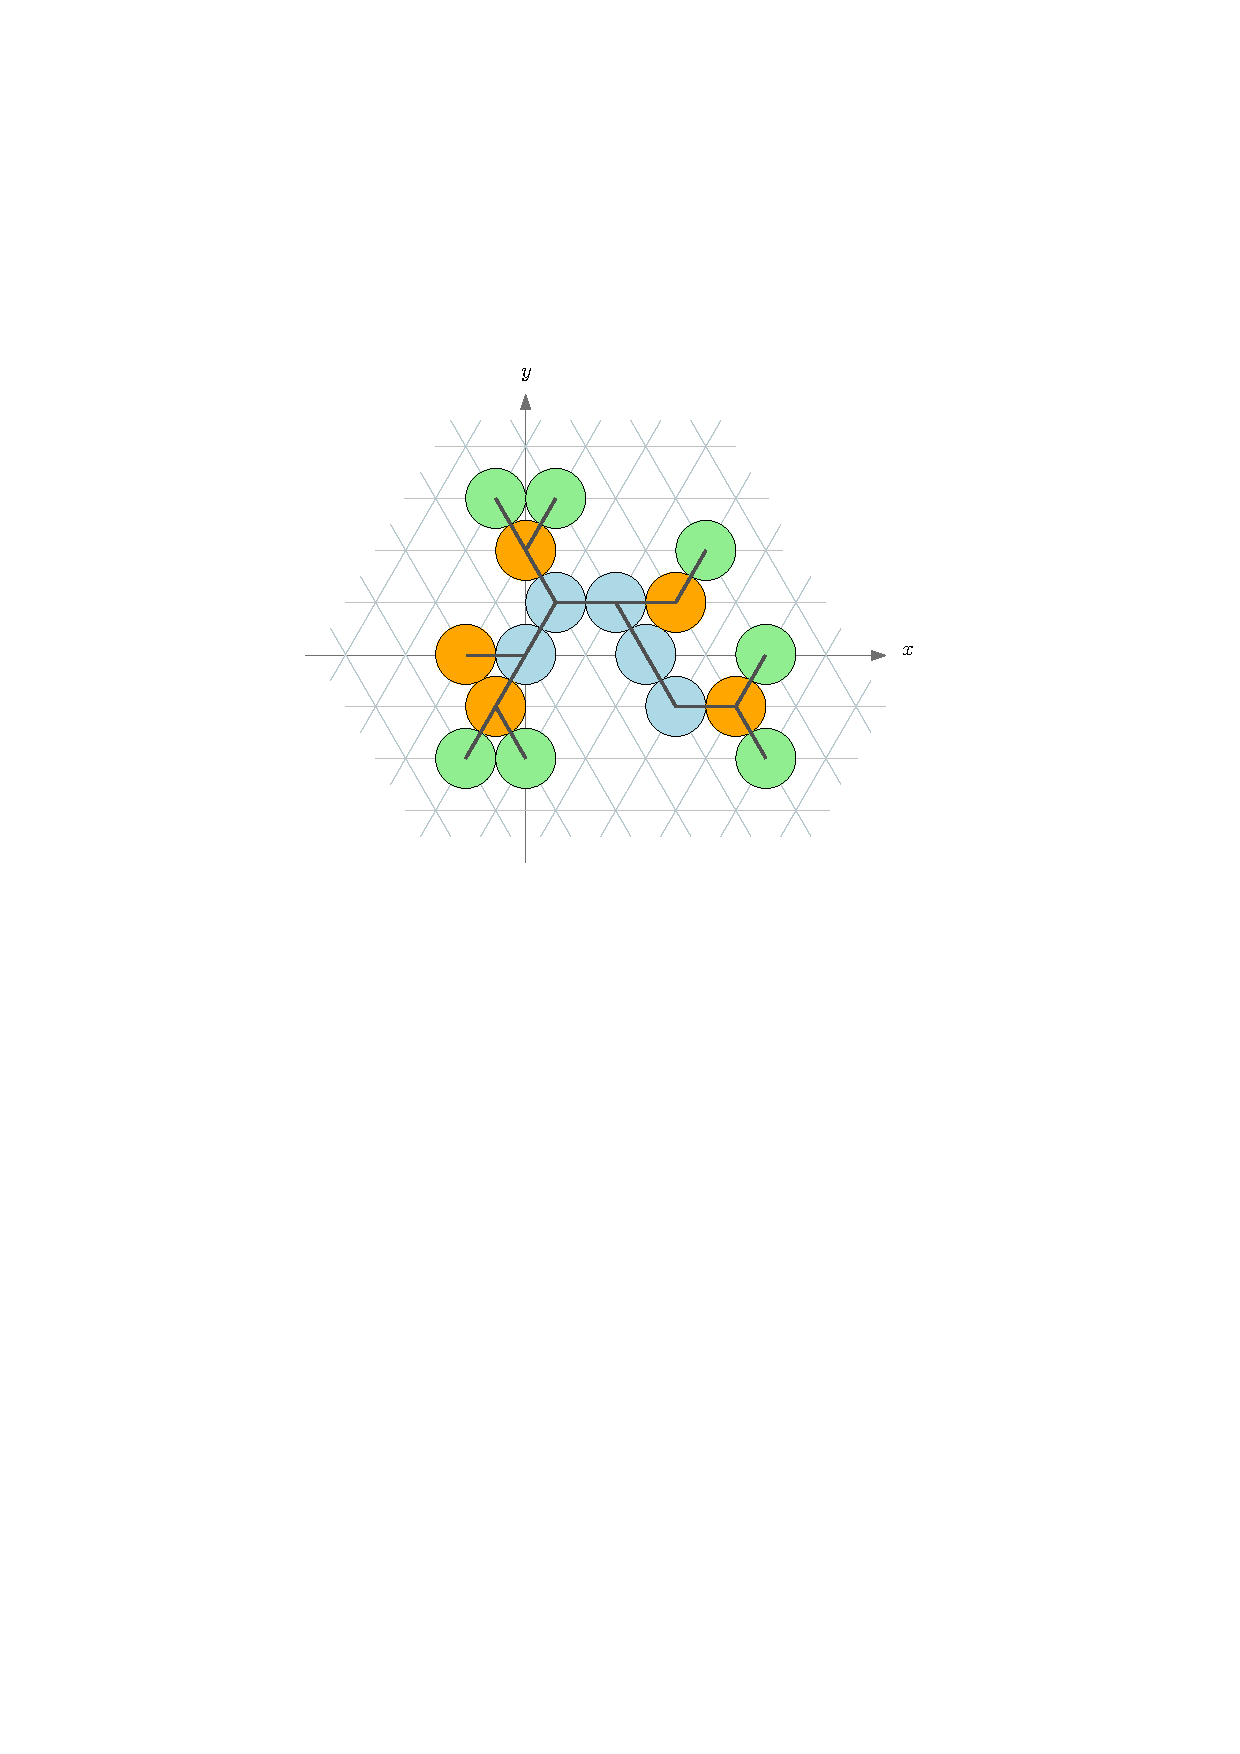
\includegraphics{graphics/ch2_tri-grid_x-monotone.pdf}
    \caption{A tri-grid x-monotone UDC representation of a lobster. The spine, although it bends twice, is embedded on strictly increasing x-coordinates.}
    \label{fig:ch2_tri-grid_x-monotone}
\end{figure}

\soeren[inline]{Everything below here needs to be restructured. The Conjectures shouldn't be in this preliminaries section. Or at least I would change the way things are introduced here. So before stating the conjecture, first define the trigrid representation on its own, as well as the concept of an $x$-monotone representation. The idea is the you defined these terms before you use them in the conjectures. Then I would not formulate them as conjectures at all, since a conjecture usually means 'We looked into this, we have an inclination but at the end of this publiucation we can not prove it.' Here I think 'Question' would be the right term. HERE WE SHOULD DISCUSS HOW TO STRUCTURE EVERYTHIng. But that seems easier in person}
\peter[inline]{Restructured preliminaries ready for next review.}

\soeren[inline]{Reihenfolge: Spined graphs, then DG, define UDG and weak DG as special cases. Define recognition question for UDG and weak UDG. Then define trigrid UDR (including neighborhood) and what a monotone UDR (including monotone neighborhood) is. Then define problem 3 as weak trigrid monotone UDG recognition. Finally state that it is unclear if every spined graph that admits a wUDR also admits a monotone one on the grid. Be specific about caterpillars and lobsters in related work.}
\peter[inline]{about right}



\chapter{Related Work}
\label{chp:related-work}

The aforementioned circle packing theorem~\cite{Koebe1936} should be considered as a fundamental result from which various research into contact graphs derives. We can categorize the topic by different aspects. Consider as an exemplary overview:

\begin{itemize}
    \item by graph class: planar, outerplanar, tree, lobster, caterpillar, ...
    \item by embeddedness: free (only the graph itself is given), embedded (an embedding is prescribed)
    \item by shape: disk, (rectilinear) polygon and many more
    \item by notion of contact: intersecting, strict, weak
    \item by problem/question and associated complexity
\end{itemize}

% Felsner~\cite{Felsner2013} describes conditions and an algorithm for rectangular contact.

Any 4-connected, internally triangulated graph admits a contact representation using rectangles~\cite{kozminski_rectangular_1985}. For some shapes, like rectilinear polygons, the problem is not so much in the representation of any planar graph under the shape constraints. Instead, we want to know the maximum complexity of the shape that is necessary to represent the graph. If the graph is planar triangulated, it admits a weighed contact representation using rectilinear polygons with at most 8 vertices: ``T-shapes''~\cite{alam_computing_2013}.

Breu and Kirkpatrick~\cite{Breu1998} showed the first complexity result that specifically applies to unit disk graphs. They introduce the topic by showing that recognition of \emph{intersection} graphs, in which adjacent disks' interiors may overlap, is NP-hard. Since contact graphs are just restricted intersection graphs, it follows that unit disk contact is also NP-hard to recognize in general.

On the other hand, it has been shown by Klemz et al.~\cite{Klemz2015} that the recognition problem for caterpillars under the strict contact notion can be decided in linear time. This result is based on an observation that if two inner spine vertices of degree 5 are not separated by a spine vertex with degree at most 3 between them, the leaves are simply ``too many'' and will not fit. This property is quite easy to check. Although the result is considered questionable due to some vagueness in the proof, it remains intuitive.

With the findings of Cleve~\cite{Cleve2020}, the author turns his attention to the weak contact notion and the triangular grid. Under this notion, caterpillars can now definitely be recognized in linear time, and trees are still NP-hard.

We continue from these results with this thesis, going hand in hand with a new paper by Bhore et al.~\cite{Bhore2021}. They take the next step from the caterpillar to the slightly more complex lobster. Our particular attention concerns the proof that, assuming the x-monotonicity and triangular grid layout, these graphs can also be recognized in linear time. The method is more difficult than for caterpillars, as it requires a constructive algorithm with a dynamic programming approach---the same approach which we discuss in Chapter~\ref{ch:dynprog} and implement.

Interestingly, the recognition problem becomes harder if an embedding is prescribed in addition to the graph itself. It is even NP-hard to recognize embedded unit disk contact caterpillars under weak contact~\cite{Chiu2019}. The given embedding robs us of our choice to place the subtrees such that the spine cannot ``turn in on itself''. While the complexity of strict UDC for trees is yet unknown (but clearly no harder than NP), if the tree is embedded, it remains NP-hard~\cite{Bowen2015}.


\chapter{Dynamic Program}
\label{ch:dynprog}

We describe two algorithms that aim to decide Problem~\ref{prob:weak-udc-lobster} on a lobster instance of size $n$ in time linear in $n$. The \emph{dynamic program} is an implementation of the algorithm conceptualized in the literature~\cite{Bhore2021}, with a few refinements for practical performance. It solves Problem~\ref{prob:weak-udc-lobster} exactly, i.e. if and only if the lobster admits a tri-grid x-monotone embedding, the dynamic program decides on ``yes'' as its output.

Dynamic programming is a technique whereby a problem is solved by dividing it into smaller sub-problems and combining their solutions.
A key feature of this approach is the reuse of solutions to sub-problems which emerge in different problem divisions.

%\begin{figure}
%     \centering
%     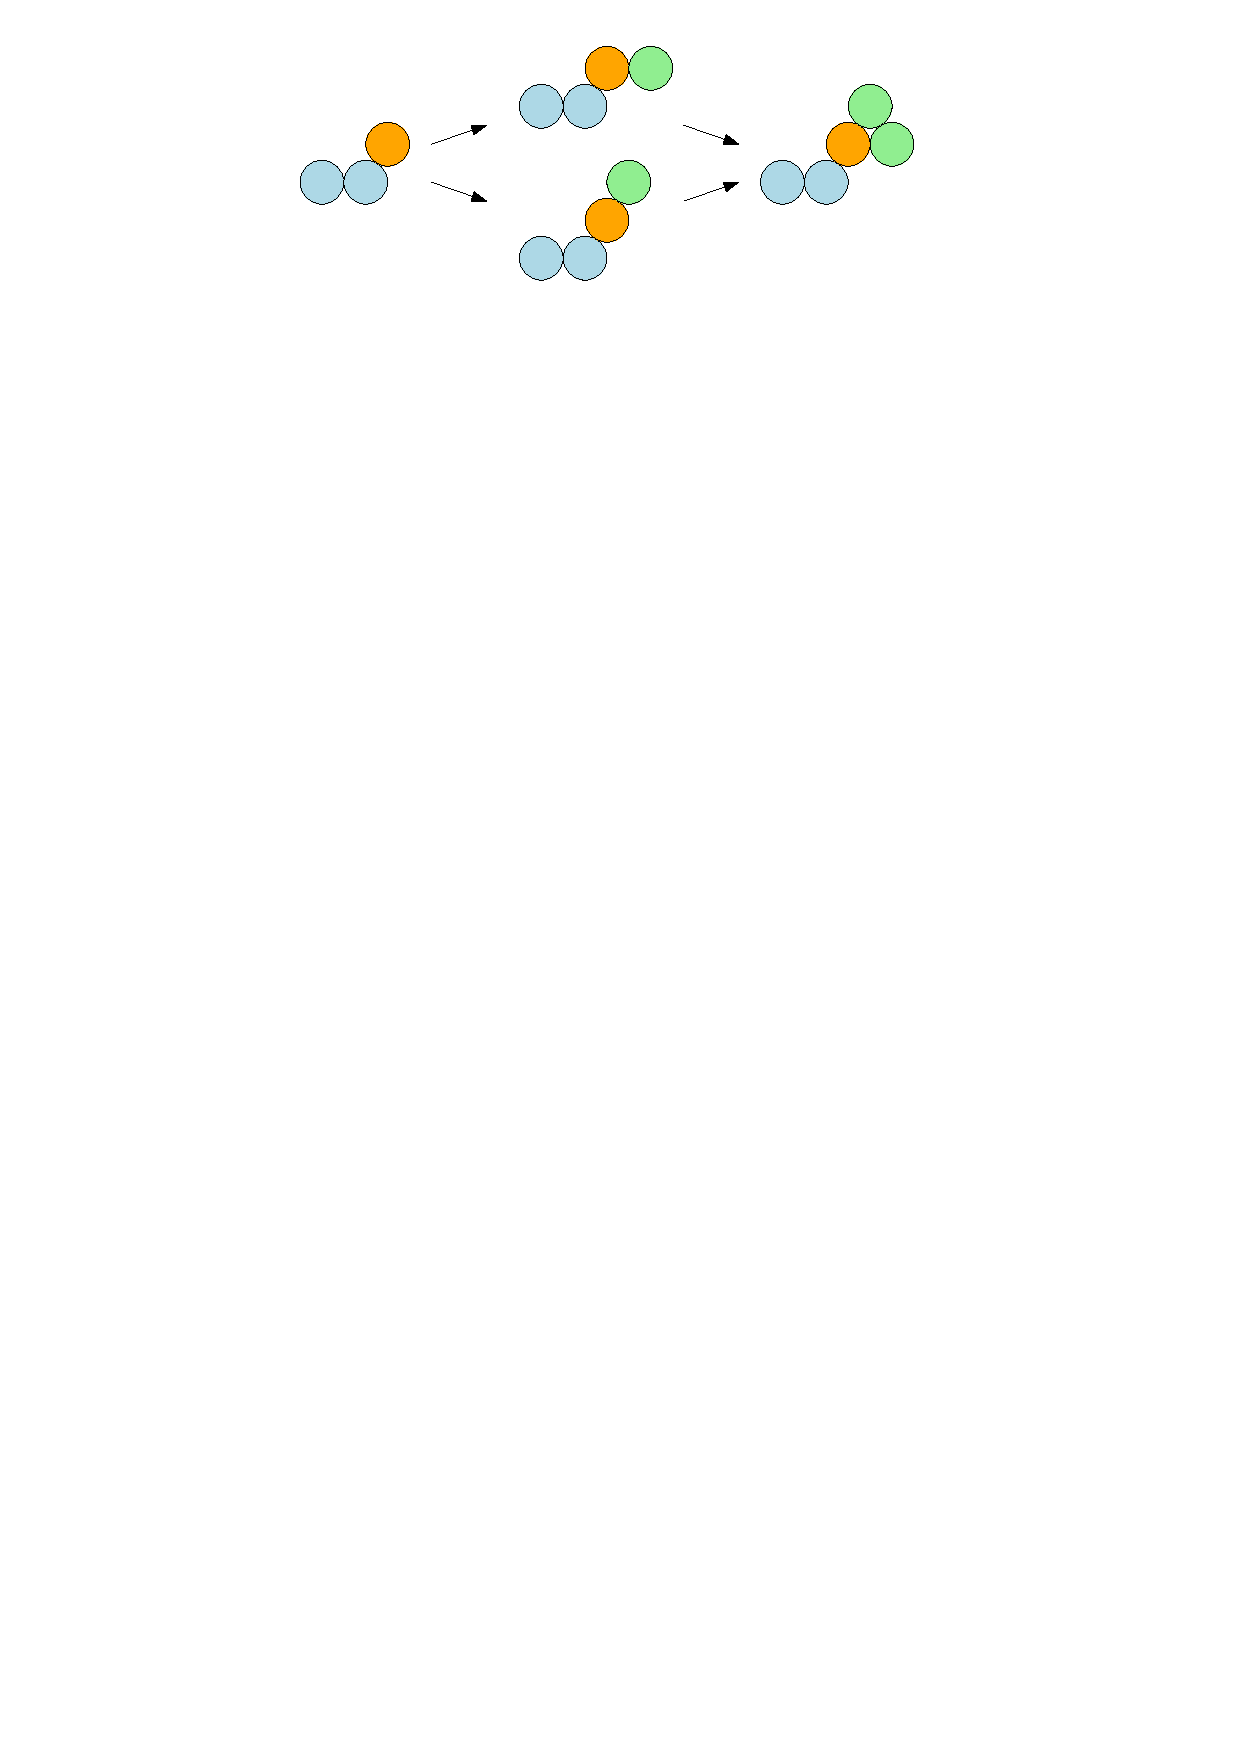
\includegraphics{graphics/ch4_reuse.pdf}
%     \caption*{Problem reuse in the dynamic program. The disk configurations represent some partial UDC representations of a lobster corresponding to partial problems. These result from decisions of the dynamic program during subdivision. A partial problem subdivides into several partial problems, among them the ones following the arrows.
%     Note that the representation on the right side results from subdivision of different problems. The key to the efficiency of the dynamic programming approach is that we solve this problem at most once, even though we may encounter it from multiple predecessors. We can reuse its answer to answer both the sub-problems in the middle.
%     In other words, we only remember one unique copy of the signature for the new partial problem.
%     }
%     % \label{fig:ch4_reuse}
% \end{figure}

\section{Problem Definition}
\label{section:ch4-probdef}
To apply the dynamic programming idea to Problem~\ref{prob:weak-udc-lobster}, we must extend its definition to that of the \emph{partial recognition problem} which we introduce in this section.

\begin{figure}[b]
    \centering
    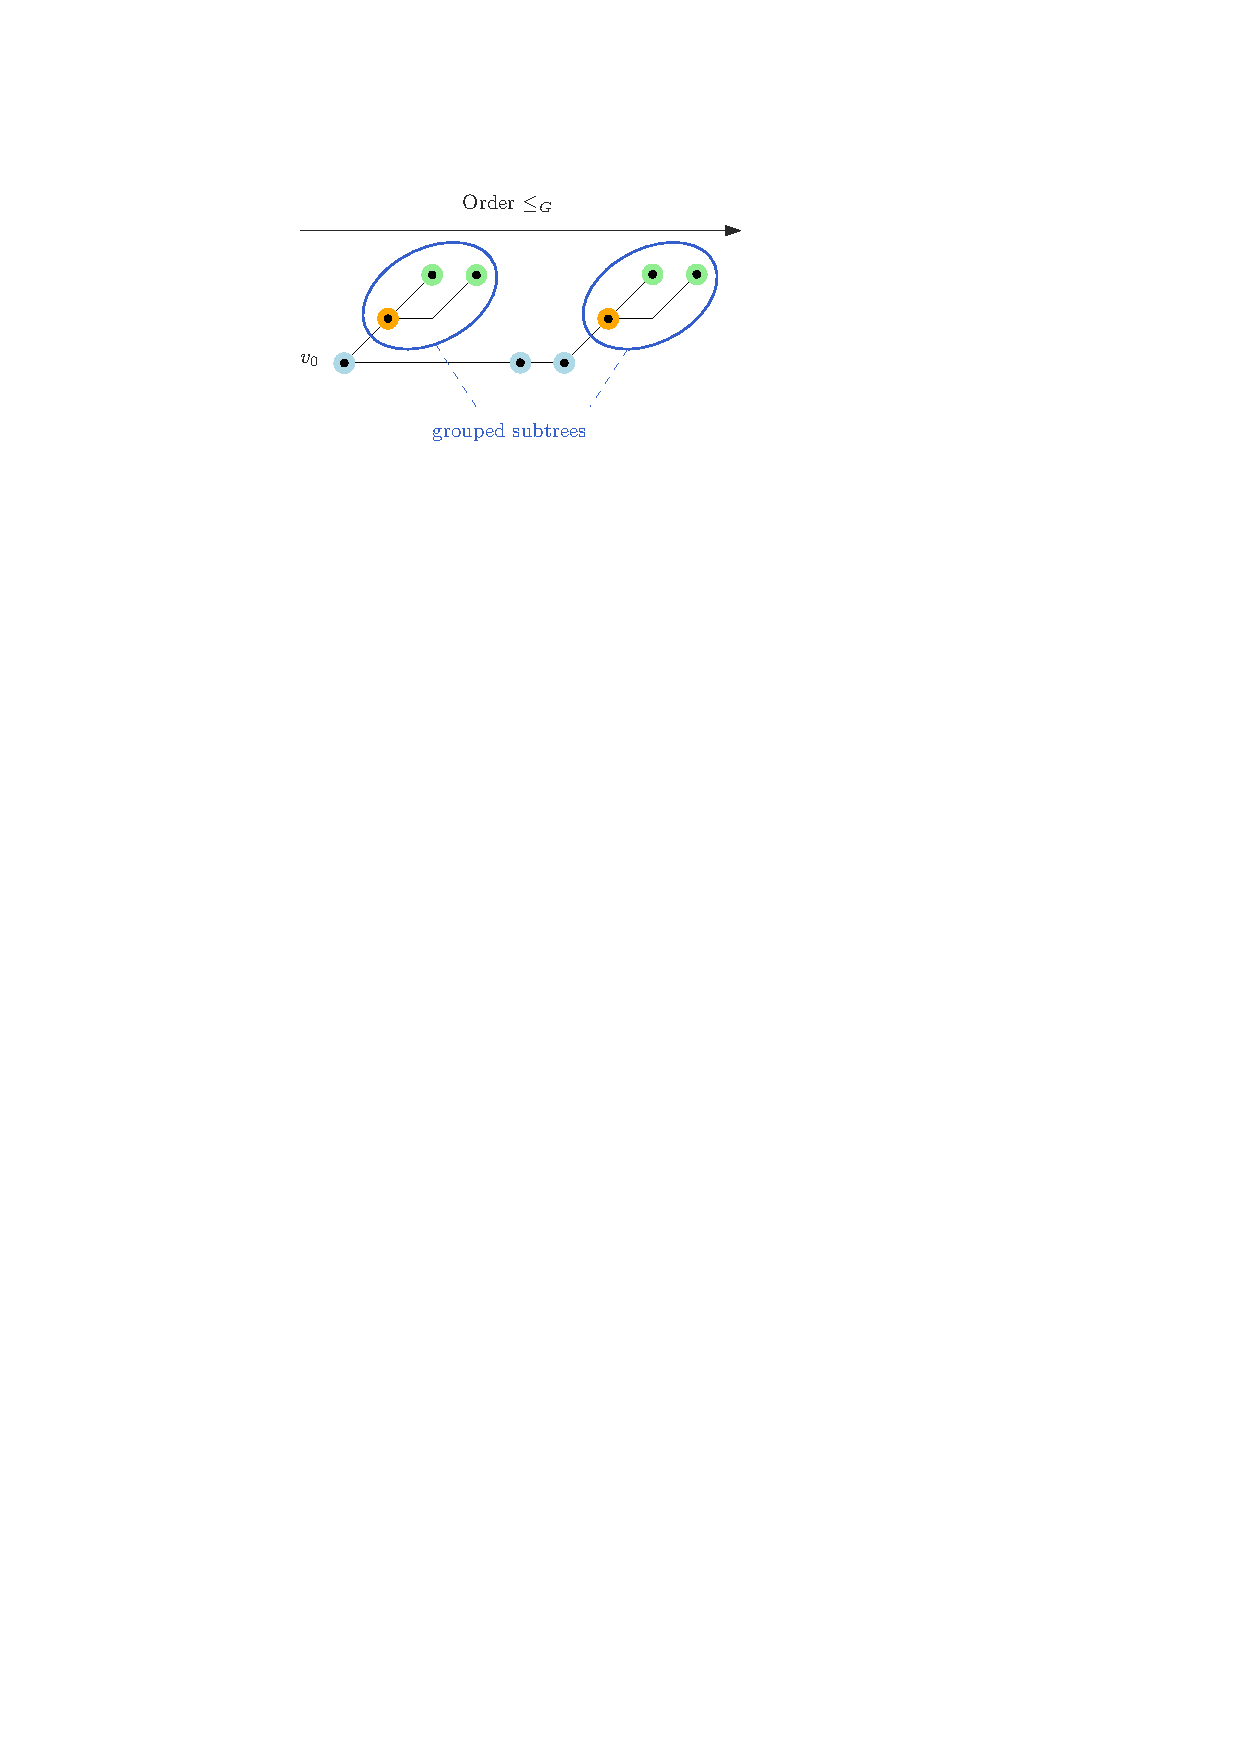
\includegraphics{graphics/ch4_order.pdf}
    \caption[Admissible order]{An admissible order over $V$, from left to right.}
    \label{fig:ch4-order}
\end{figure}

Let $G = (V, E), V = \Spines \dotcup \Branches \dotcup \Leaves$ be a lobster. 

The \emph{embedding order} $\order$ for $G$ is a total order over $V$. It dictates the order in which the algorithm assigns coordinates to vertices in its exploration of the partial problem space. Starting from the initial problem, where no vertices are embedded, the minimum vertex under $\order$ is assigned coordinates first. The final coordinate assignment to the maximum vertex implies an affirmative answer to the original problem instance.

An embedding order $\order$ is \emph{admissible} if it fulfills the following criteria.

\begin{itemize}
    \item $\order$ is a total order. It is reflexive, transitive and antisymmetric.
    \item $\order$ orders the spine.
    \begin{itemize}
        \item There exists a minimal $v_0 \in \Spines$, i.e. $\forall v \in V: v_0 \order v$, which is connected to at most one other spine.
        \item Let $s_1 \neq s_2 \neq s_3 \in \Spines, s_1 \order s_2, s_1 \order s_3$ and $(s_1, s_3) \in E$. Then $s_3 \order s_2$.
    \end{itemize}
    \item $\order$ groups branches together with their parent spine. Let $s_1, s_2 \in \Spines, b \in \Branches, s_1 = p(b)$ and $s_1 \order s_2$. Then $b \order s_2$.
    \item $\order$ groups subtrees together. Let $l \in \Leaves, b = p(l) \in \Branches, v \in V, (b, v) \not\in E$ and $b \order v$. Then $l \order v$.
    \item Parent vertices come first. Let $v_1, v_2 \in V$. If $v_1 = p(v_2)$, then $v_1 \order v_2$.
\end{itemize}

Figure~\ref{fig:ch4-order} shows a possible embed order $\order$, which adheres to these criteria.

For a given lobster, there may be multiple possible admissible orders. Whichever one we choose, the dynamic program requires that the chosen order definition remains fixed during the execution of the algorithm across all partial problem instances.

The \emph{depth} $\depth$ of a partial problem is the number of embedded vertices, i.e. the $\depth$ smallest vertices under $\order$. It takes $\depth$ subdivisions from the initial partial problem to arrive at a (set of) depth $\depth$ problems.

Let $V = V_d \dotcup V_r$ be a bipartition of $V$ ordered under an order $\order$, where the \emph{prefix} $V_d$ contains the smaller vertices until some cutoff vertex and $V_r$ contains the remaining larger vertices: $$\forall v_d \in V_d, v_r \in V_r: v_d \order v_r.$$ We call $V_d$ the set of ``embedded'' vertices, meaning that we have, before fully defining the entire embedding function $d\colon V \to \reals^2$, already decided on some $d(v)$ for every $v \in V_d$. $V_r$ are then the remaining vertices yet to be embedded. For a partial problem with depth $\depth$, $|V_d| = \depth.$

The \emph{spine head} $\coord_s$ is the coordinates of the last embedded spine vertex and the \emph{branch head} $\coord_b$ is the coordinates of the last embedded branch vertex. At depth $\depth$, 

\begin{equation*}
\begin{aligned}
\coord_s &= \mathrm{max}_{\order}(v \in V_d \cap \Spines) \text{ and} \\
\coord_b &= \mathrm{max}_{\order}(v \in V_d \cap \Branches).
\end{aligned}
\end{equation*}

Let $\coord$ be the tri-grid embedding coordinates of a spine vertex. The \emph{fundamental neighborhood} of a partial problem 
\[
\Phi(\coord_s) = \left\{ \coord_s + \left(x + \frac y2, \frac{\sqrt3}2 y\right) \,\middle|\,|x + y| \leq 2; x, y \in \mathbb Z \right\}
\]
is a region of interest for avoiding potentially conflicting assignments of coordinates to vertices in $V_r$. It defines a ``perceivable range'' inside of which the algorithm remembers the embedding coordinates of vertices in $V_d$ and are also potential embedding coordinates of vertices in $V_R$.

\begin{figure}
    \centering
    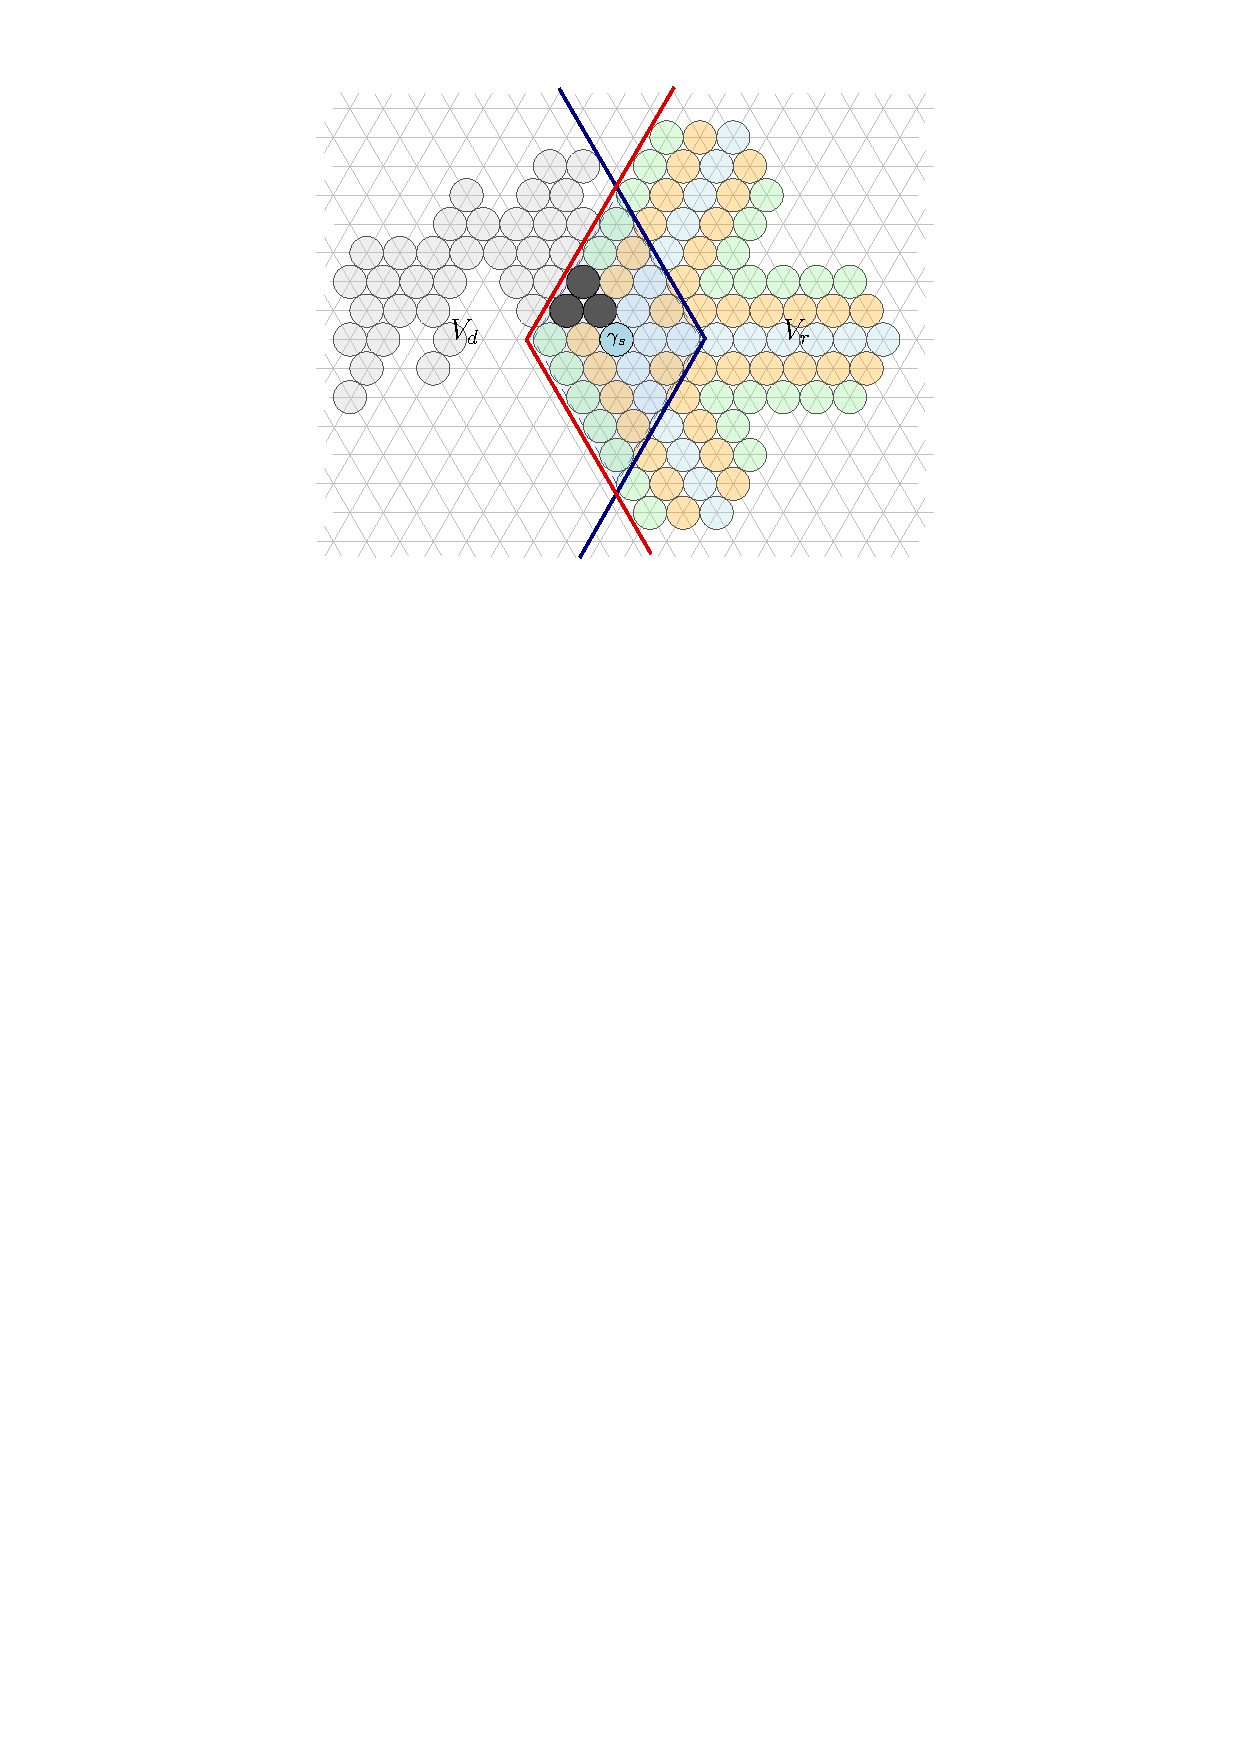
\includegraphics{graphics/ch4_reach.pdf}
    \caption[Motivation for the fundament $F$]{Motivation for the fundament $F$. We can imagine vertices from $V_d$ embedded in parent problems, illustrated here in translucent grey. Future $V_r$ coordinates may lie anywhere to the right, with some exemplary coordinates shown for the spine laid out only upwards, downwards or straight. The possible areas for past and future vertex coordinates are delineated in blue and red respectively, and the intersection of the areas is the fundamental neighborhood $\Phi(\coord_s)$. Vertices from $V_d$ within the fundamental neighborhood form the fundament, illustrated in solid grey. We must keep track of them for potential conflicts in coordinate assignment.}
    \label{fig:ch4_reach}
\end{figure}

The \emph{fundament} $F \subseteq \Phi(\coord_s)$ is a subset of local grid locations which are unavailable due to being reserved for vertices in $V_d$. Figure~\ref{fig:ch4_reach} visualizes this reasoning.

The \emph{signature} $\signature$ of a partial problem is the tuple $(\depth, \coord_s, \coord_b, F)$, specifying the depth, heads and fundament of the problem.

\begin{problem}[Partial UDC Recognition for Lobsters]
Given a Lobster $G$, an embedding order $\order$ and a signature $\signature$, does $G$ admit a partial tri-grid x-monotone embedding of the remaining vertices under the constraints defined by $\signature$?
\label{prob:partial-udc-lobster}
\end{problem}

\begin{figure}
    \centering
    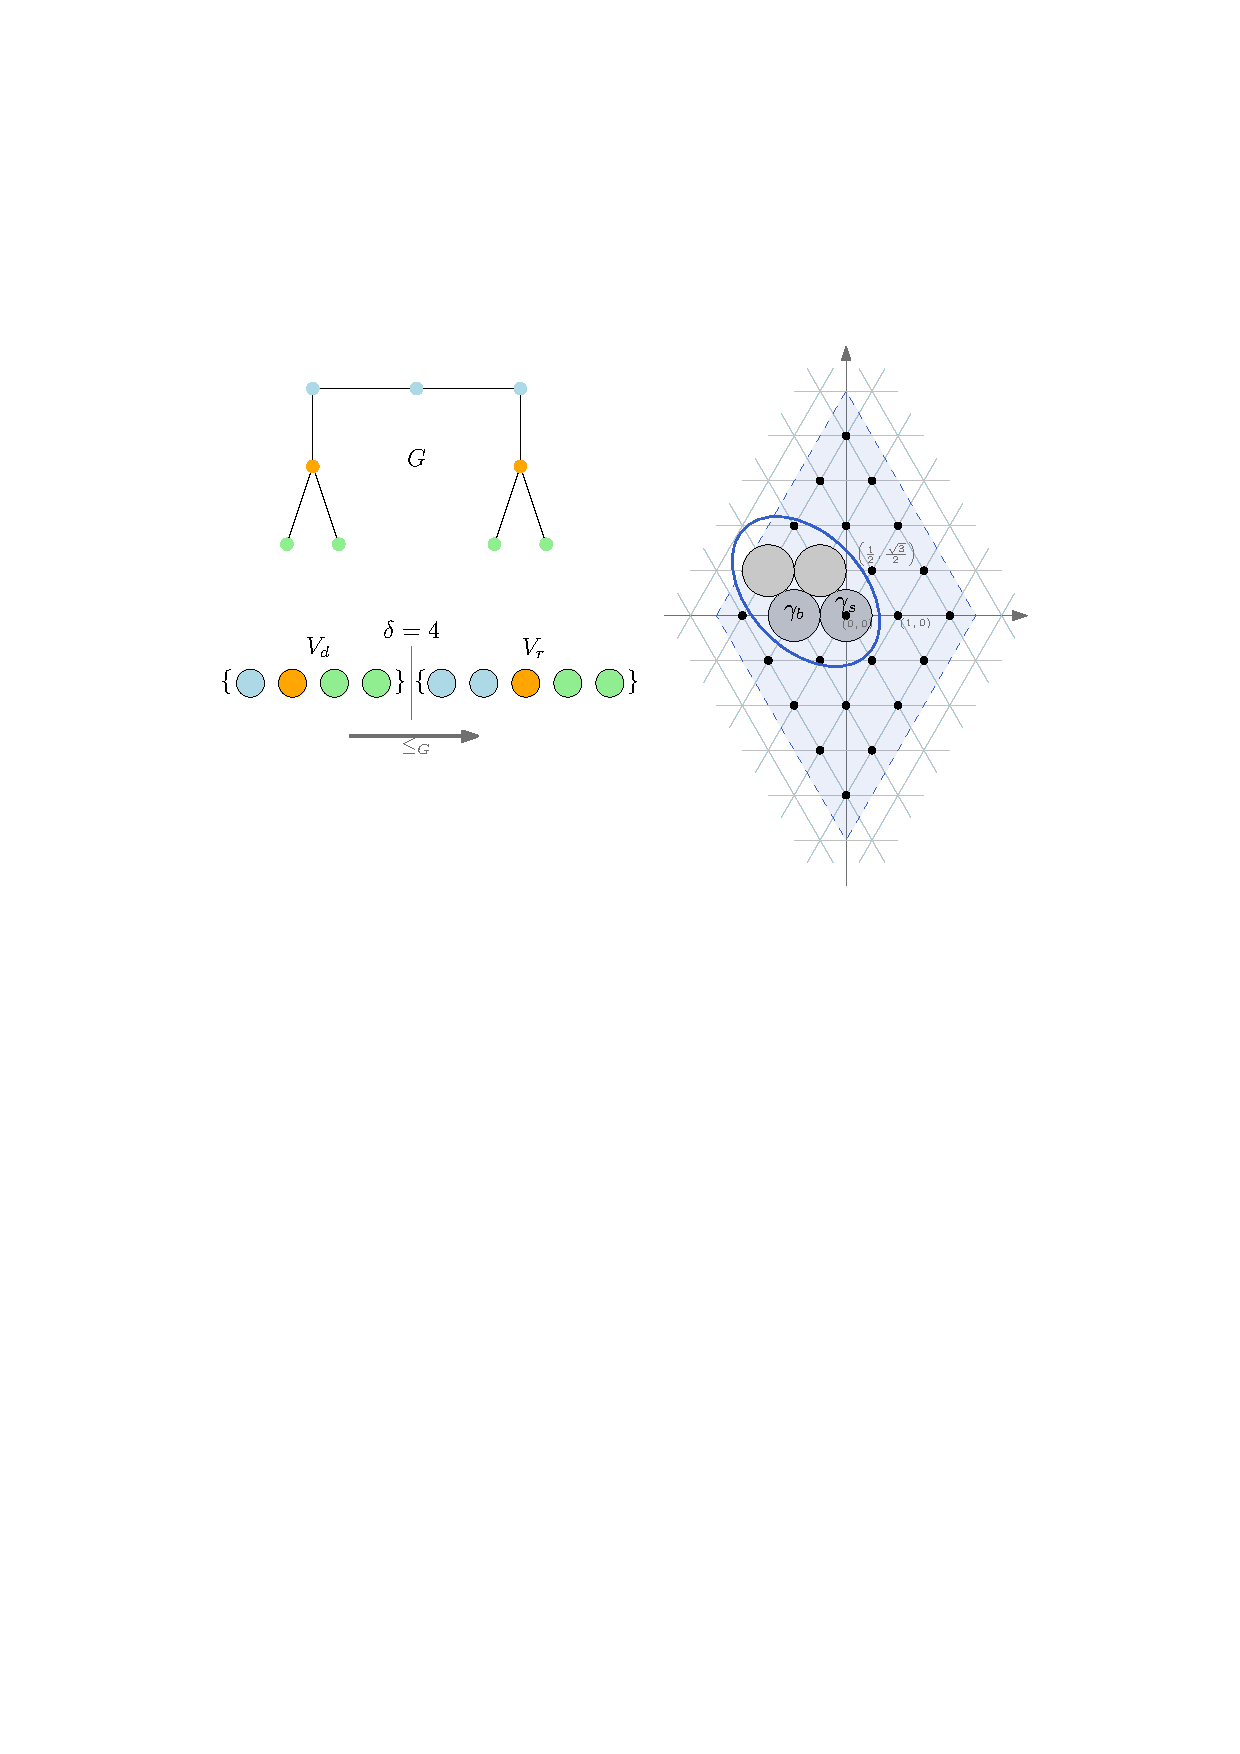
\includegraphics{graphics/ch4_partialproblem.pdf}
    \caption[Partial problem instance]{An instance of Problem~\ref{prob:partial-udc-lobster}. The task is to decide the lobster depicted in the top left as a node-link diagram. Its vertices, illustrated as disks in the bottom left, are partitioned into the prefix $V_d$ and the remainder $V_r$, with the second spine vertex to be embedded next.
    On the right side, the fundamental neighborhood $\Phi(\coord_s)$ is marked with dots on the coordinates and enclosed with a dashed line. The coordinates contained in the fundament $F$ are represented by grey disks, marked with the blue ellipse. These locations are earmarked for the embedding of the vertices in $V_d$ and no longer available for any vertex in $V_r$.}
    \label{fig:ch4_partialproblem}
\end{figure}

Refer to Figure~\ref{fig:ch4_partialproblem}, which visualizes a partial problem instance, for an illustration of all the above concepts.

We are now prepared to define the dynamic programming algorithm on the extended problem definition.

\begin{algorithm}[t]
\SetKwFunction{Divide}{divide}
\SetKwFunction{Sort}{sort}
\SetKwData{V}{V}
\SetKwData{Sigs}{S}
\SetKwData{sig}{$\signature$}
\SetKwData{parent}{parent}
\SetKwData{undef}{undef}
\SetKwData{Fundament}{F}
\KwIn{lobster $G = (V, E), V = \Spines \dotcup \Branches \dotcup \Leaves$}
\KwOut{``yes'' if $G$ admits a tri-grid x-monotone embedding, ``no'' otherwise}
$n \gets |V|$\;
\V $\gets \Sort(V)$ \tcp*{establish some admissible order $\order$}
$\Sigs_0 \gets \{ \text{initial signature: } (\depth=0, \coord_s=\undef, \coord_b=\undef, \Fundament = \emptyset) \}$\;
\For{$\depth = 1$ \KwTo $n$}{
    $\Sigs_\depth \gets \bigcup\limits_{\sig \in \Sigs_{\depth-1}}$ \Divide{$\V, \sig$}\;
}
\If{$\Sigs_n = \emptyset$}{
    \Return{``no''}\;
}
\Else{
    \Return{``yes''}\;
}
\caption[Simplified dynamic program]{The simplified dynamic program. This scheme does not implement the run-time efficiency improvements discussed later in this chapter, but it serves to illustrate the dynamic programming formula and the reasoning behind its linear-time complexity.}
\label{alg:simple-dynprog}
\end{algorithm}

If we can construct any partial problem instance $\probinst$ at the maximum depth $\depth = |V|$, there are no further vertices to embed and the answer is always ``yes'' (the input lobster does admit a tri-grid x-monotone embedding). From the set $\DataSty{S}_\depth$ of all partial problem instances at depth $\depth < |V|$ reachable by subdivision, the answer is ``yes'' if there exists a sub-problem yes-instance of some $\probinst \in \DataSty{S}_\depth$, and ``no'' only if no descendant instance reaches the maximum depth. We therefore subdivide partial problems until we find a maximum-depth instance or until the search space is exhausted. The algorithm will be defined such that the combined assignments of coordinates during division of the instance define a total embedding function $d(G)$.

Algorithm~\ref{alg:simple-dynprog} shows an illustrative implementation. Unlike this pseudo-code, the common conception of a dynamic program involves a ``combination'' of solved sub-problems into a solution of the super-problem. Because of the above conditions on yes- and no-instances, we can short-circuit the recombination step. See Subsection~\ref{section:ch3_earlyexit} below.

\begin{algorithm}
\SetKwFunction{Divide}{divide}
\SetKwData{Candidates}{K}
\SetKwData{Candidate}{$\kappa$}
\SetKwArray{V}{V}
\SetKwData{Sigs}{S}
\SetKwData{sig}{$\signature$}
\SetKwData{parent}{parent}
\SetKwData{undef}{undef}
\SetKwData{Fundament}{F}
\SetKwProg{Fn}{Function}{}{}
\Fn{\Divide{$\V, \signature$}}{
\KwIn{ordered vertices $\V = \Spines \dotcup \Branches \dotcup \Leaves$, signature $\signature = (\depth, \coord_s, \coord_b, \Fundament)$}
\KwOut{Set of signatures $\Sigs'$}

$v \gets \V{$\depth$}\;$

\If(\tcp*[f]{first vertex $\implies v \in \Spines$}){$\depth = 0$}{
    $\coord_s' \gets (0, 0)$\;
    $\Fundament' \gets \{ \coord_s' \}$\;
    \Return{$\{ (1, \coord_s', \undef, \Fundament') \}$}\;
}

$\Sigs' \gets \emptyset$\;

\If(\tcp*[f]{spine vertex}){$v \in \Spines$}{
    $\Candidates \gets \Gamma^{x+}(\coord_s) \setminus F$\;
    \ForEach{$\kappa \in \Candidates$}{
        $\Fundament' \gets (\Fundament \cap \Phi(\kappa)) \cup \{ \kappa \}$\;
        $\signature \gets (\depth+1, \kappa, \undef, \Fundament')$\;
        $\Sigs' \gets \Sigs' \cup \{ \signature \}$\;
    }
}
\ElseIf(\tcp*[f]{branch}){$v \in \Branches$}{
    $\Candidates \gets \Gamma(\coord_s) \setminus F$\;
    \ForEach{$\kappa \in \Candidates$}{
        $\Fundament' \gets \Fundament \cup \{ \kappa \}$\;
        $\signature \gets (\depth+1, \coord_s, \kappa, \Fundament')$\;
        $\Sigs' \gets \Sigs' \cup \{ \signature \}$\;
    }
}
\Else(\tcp*[f]{leaf})
{
    $\Candidates \gets \Gamma(\coord_b) \setminus F$\;
    \ForEach{$\kappa \in \Candidates$}{
        $\Fundament' \gets \Fundament \cup \{ \kappa \}$\;
        $\signature \gets (\depth+1, \coord_s, \coord_b, \Fundament')$\;
        $\Sigs' \gets \Sigs' \cup \{ \signature \}$\;
    }
}

\Return{$\Sigs'$}\;

}
\caption[Subdivision of partial problem instances]{Subdivision of partial problem instances. We deal with partial problems in terms of their signatures, which contain the distinguishing properties of the instance.
Dividing an instance consists of assigning the next vertex in order to one of the \emph{candidate coordinates} in \DataSty{K} relative to the appropriate (spine- or branch-) head. Each possibility becomes a sub-instance. We maintain the fundament \DataSty{F} and the heads $\coord_s$ and $\coord_b$ as appropriate, depending on the type of assigned vertex.
Recall that $\Gamma(\coord)$ and $\Gamma^{x+}(\coord)$ define the tri-grid (x-monotone) neighborhood of $\coord$.}
\label{alg:divide}
\end{algorithm}

Algorithm~\ref{alg:divide} describes the subroutine by which descendant partial problems are derived. It returns fewer than six partial embedding sub-instances (with the negligible sole exception of $\depth = 1$).

\begin{figure}
    \centering
    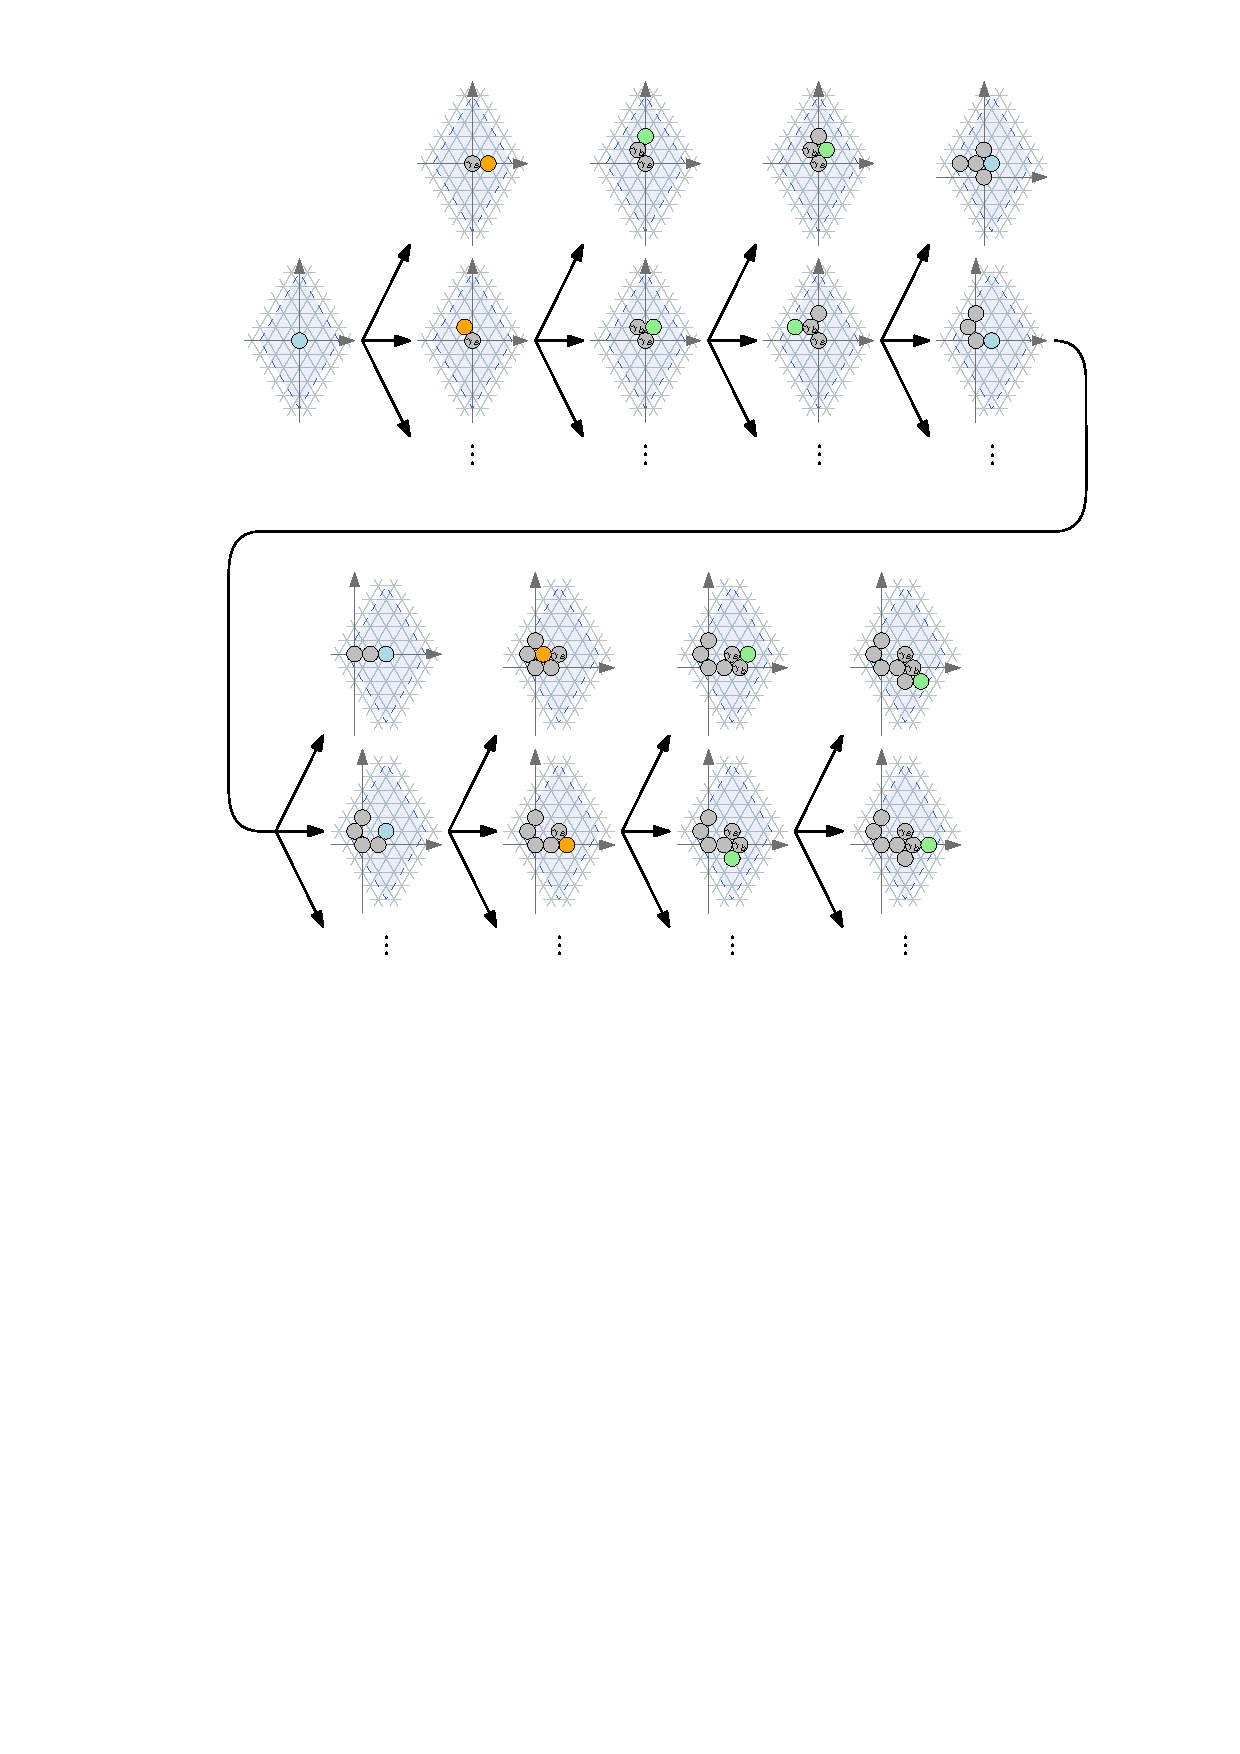
\includegraphics{graphics/ch4_dpexample.pdf}
    \caption[Dynamic program example]{This might be the path through the search space visited by the dynamic program to solve a lobster. Each of the small drawings represents one signature. The fundamental neighborhood $\Phi(\coord_s)$ is enclosed in dashed blue. The disk of the most recently assigned vertex bears the color of its type: blue for spines, orange for branches and green for leaves. Gray disks represent coordinates in the fundament $F$. The spine and branch heads $\coord_s$ and $\coord_b$ are also labeled, if relevant and not implied by color. The view always centers on $\coord_s$, the center of $\Phi(\coord_s)$. The black arrows signify construction of the partial problem associated with the target signature by subdivision of the source problem.}
    \label{fig:ch4_dpexample}
\end{figure}

Figure~\ref{fig:ch4_dpexample} shows how the dynamic program might arrive at a decision given the same lobster as in Figure~\ref{fig:ch4_partialproblem}. The arrows represent \texttt{divide} operations, yielding different paths forward. The colored disk marks the chosen candidate for the current embedding coordinates. At each point, the local knowledge of the fundament exactly suffices to prevent us from considering invalid duplicate assignments of coordinates.

Given a lobster $G = (V, E)$, we can construct an initial partial UDC problem signature $\signature$ as illustrated in Algorithm~\ref{alg:simple-dynprog}.
The dynamic programming algorithm answers Problem~\ref{prob:weak-udc-lobster} on $G$.\cite{Bhore2021}

\section{Complexity}

\begin{theorem}
Let $G = (V, E)$ be a lobster with $|V| = n$. Algorithm~\ref{alg:simple-dynprog} runs in time $O(n)$.
\end{theorem}

\begin{proof}
The determination of $\order$ and the ordered vertex set \DataSty{V} is possible in time $O(|V|)$ simply by traversing $G$ from a suitable starting spine $v_0$ of our choice (front or back).

The algorithm constructs an initial partial UDC problem signature, from which all sub-problem signatures are derived. Each problem is either \texttt{divide}-d further or outright solved in constant time simply by having maximum depth. Also, due to the memory of problems already encountered, no problem is processed more than once. It therefore suffices to show that the number of signatures under consideration is bound by $O(n)$.

In fact, the size of the set of signatures $\DataSty{S}_\depth$ that may possibly occur at any particular depth $0 \leq \depth \leq n$ is bound, due to our representation of signatures, by a constant. Consider the constituent components of the signatures at depth $\depth$.

\begin{itemize}
    \item The spine head $\coord_s$ does not contribute to the quantity of instances. The problem is translation-invariant. We can always derive an equivalent instance by translating $\coord_s$ to the origin point, and $\coord_b$ and $F$ with it.
    \item The branch head $\coord_b$ is relevant only when the vertex to be embedded next is a leaf, due to the subtree grouping property of $\order$. Even in that case, its position is limited to at most 6 coordinates relative to $\coord_s$.
    \item $F$ is limited to be a subset of $\Phi(\coord_s)$ and therefore to the constant amount of $2^{|\Phi(\coord_s)|} = 2^{25}$ values.
\end{itemize}
%\soeren[inline]{You could make this explicit as $n\cdot 1 \cdot 6 \cdot 2^{25} \in \mathcal{O}(n)$. Actually I am unsure if this helps the understanding.}

Since all constituent components of signatures at depth $\depth$ are limited to a constant-bound set of values and we discard duplicate signatures, the number of signatures at depth $\depth$ is also constant-bound and the total number of sub-problems is in $O(n)$. A single problem (signature) takes a constant amount of time to handle, putting the total run time in $O(n)$ as well.
\end{proof}

This result superficially seems to declare Problem~\ref{prob:weak-udc-lobster} as tractable. However, the constant bound $C$ for the number of equi-depth instances is too high to ignore for practical applications. On its face, it may be as high as

\begin{equation*}
    C = 5 \cdot 2^{24} = 83,886,080
\end{equation*}

In this first estimate, we consider 5 locations for the branch head relative to the spine head and the spine disk before it, which eliminates one coordinates option. At depth $d>0$, $F$ always contains $\coord_s$, leaving us with just 24 potentially unavailable coordinates.

\section{Run-Time Improvements}

Consider the high constant bound $C$ of sub-problem signatures at some arbitrary depth. Upon further consideration of the algorithm definition, not every value from the domain of $\coord_b$ and $F$ can occur in real problems. Our estimate for the value of $C$ should drop accordingly. We also discuss several improvements to the algorithm which reduce the run time in practice. Some of them are based on recognizing \emph{equivalence} of signatures.

Let $\probinst_1$ with signature $\signature_1 = (\depth, \coord_s^1, \coord_b^1, F^1)$ and $\probinst_2$ with signature $\signature_2 = (\depth, \coord_s^2, \coord_b^2, F^2)$ be two partial recognition problem instances on the lobster $G = (V, E), |V| = n$. Let $V_r \subseteq V$ be the vertices remaining without coordinates assignment---equivalently, the largest $n-\depth$ vertices under the order $\order$.

$\probinst_1$ and $\probinst_2$ are \emph{equivalent} if and only if for any witness embedding function $d_1\colon V_r \to \reals^2$ that certifies a yes-answer to $\probinst_1$, we can transform it into a yes-witness $d_2$ for $\probinst_2$ and vice-versa by translation and mirroring of the coordinates.

The global \emph{breadth} $\overline{m}$ of the graph class of lobsters is the maximum number of equivalence classes that occur at any depth over all lobsters by application of Algorithm~\ref{alg:simple-dynprog}. This is important because the run time in practice is bound by $\overline{m} \cdot n$.

The improvements described here feature in Algorithm~\ref{alg:improved-dynprog}, which corresponds to the actual implementation used for our experiments in Chapter~\ref{ch:evaluation}.

\subsection{Early Exit}
\label{section:ch3_earlyexit}

Our definition of the partial problem includes that the combined answer is ``yes'' iff any sub-problem answer is ``yes''. Once we find a positive instance, we can instantly skip over all other sub-problems and declare the original decision problem instance solved in the affirmative.

We encourage the fast determination of this result by always prioritizing sub-problems of higher depth before sub-problems of lower depth. We augment Algorithm~\ref{alg:simple-dynprog} with one lookup data structure of encountered (``closed'') signatures at every depth and a priority queue of pending (``open'') signatures. This allows us to customize the order of processed signatures while retaining the dynamic program benefit of not duplicating computations.

The early exit strategy does not improve the time to solve a negative instance. The algorithm is forced to check every possibility until it confirms the negative answer.

\subsection{Mirror Instance}

Let $\probinst_1$ and $\probinst_2$ be two problem instances with signatures which differ only in the branch heads $\coord_b^1$ and $\coord_b^2$ and in the fundaments $F_1$ and $F_2$. Without loss of generality, we assume that $\coord_s^1 = \coord_s^2 = (0, 0)$.
Let $m((x, y)) = (x, -y)$ be the function that mirrors coordinates along the x-axis.
Then $\probinst_1$ is equivalent to $\probinst_2$ if $\coord_b^1 = m(\coord_b^2)$ and $F_1 = \{m(\coord) \mid \coord \in F_2\}$.
This effectively cuts $\overline{m}$ in half.

\subsection{Reachability}

Define the \emph{reach} $R$ of the partial problem instance $\pi$ as the set of all possible future embedding coordinates---in other words, the union of all candidate sets $K$ of all descendent sub-problem instances.

Then the unreachable coordinates $\Phi(\coord_s) \setminus R$ have no more bearing on the answer of the problem. We may as well disregard all unreachable coordinates in $\Phi(\coord_s)$ by just assuming that they are in the fundament, i.e. unavailable.

Construct an instance $\pi'$ equal to $\pi$, except for the fundament $F' = F \cup (\Phi(\coord_s) \setminus R)$. Then $\pi$ is equivalent to $\pi'$, and so are any other instances that differ only in the availability of unreachable coordinates.

\subsection{Domination}

Let $\probinst_1$ and $\probinst_2$ be two otherwise equal problem instances with fundaments $F_1$ and $F_2$. If $F_1 \subseteq F_2$, then $\probinst_1$ allows as many or more options for future coordinates candidates of vertices in $V_R$ than $\probinst_2$. $\probinst_1$ is easier to recognize than $\probinst_2$, and we say that $\probinst_1$ \emph{dominates} $\probinst_2$.

We can use the resulting hierarchy of instances to instantly disregard a sub-problem under consideration if, looking at the memory of known solutions with equal depth and equal $(\coord_b-\coord_s)$, we find that we have already decided a dominating instance as a ``no''. Attempting the harder instance will never result in a ``yes''-answer.

\begin{algorithm}
\SetKw{New}{new}
\SetKw{Not}{not}
\SetKwFunction{Divide}{divide}
\SetKwFunction{Queue}{Queue}
\SetKwFunction{Priority}{priority\_predicate}
\SetKwFunction{DeMirror}{demirror}
\SetKwFunction{ApplyReachability}{apply\_reachability}
\SetKwFunction{Insert}{insert}
\SetKwFunction{Pop}{pop}
\SetKwFunction{Empty}{empty}
\SetKwFunction{ContainsDominating}{contains\_dominating}
\SetKwData{Candidates}{K}
\SetKwData{Candidate}{$\kappa$}
\SetKwData{V}{V}
\SetKwData{Sigs}{S}
\SetKwData{sig}{$\signature$}
\SetKwArray{Closed}{C}
\SetKwData{parent}{parent}
\SetKwData{undef}{undef}
\SetKwData{Fundament}{F}
\SetKwProg{Fn}{Function}{}{}
\KwIn{lobster $G = (V, E), V = \Spines \dotcup \Branches \dotcup \Leaves$}
\KwOut{``yes'' if $G$ admits a tri-grid x-monotone embedding, ``no'' otherwise}
\KwData{Priority queue of open signatures \Sigs}
\KwData{Set of closed signatures \Closed}

$n \gets |V|$\;
\V $\gets$ \Sort($V$) \tcp*{establish some admissible order $\order$}
\Sigs $\gets$ \New \Queue(\Priority) \tcp*{prefer higher depth}
$\Closed{1}, \ldots, \Closed{n} \gets \emptyset$\;

\Sigs.\Insert(initial signature: $(\depth=0, \coord_s=\undef, \coord_b=\undef, \Fundament = \emptyset)$)\;

\While{$\neg \Sigs.\Empty()$}{
    \sig $\gets$ \Sigs.\Pop()\;
    \If{\sig.$\depth$ = $n$}{
        \Return{``yes''} \tcp*{early exit}
    }
    \ForEach{\sig' $\in$ \Divide{\V, $\sig$}}{
        \ApplyReachability(\sig')\;
        \DeMirror(\sig')\;
        $\ArgSty{d} \gets \sig'.\depth$\;
        \If{$\neg \Closed{d}.\ContainsDominating(\sig')$}{
            \Sigs.\Insert(\sig')\;
            $\Closed{d}$.\Insert(\sig')\;
        }
    }
}
\Return{``no''}\;
\caption[Improved dynamic program]{The improved dynamic program. The open queue \DataSty{S} prioritizes promising signatures, while the closed sets \DataSty{C} block duplicates. The algorithm preprocesses signatures to combine equivalent problems.}
\label{alg:improved-dynprog}
\end{algorithm}


\chapter{Heuristic}
\label{ch:heuristic}

We present a fast approach to decide problem~\ref{prob:weak-udc-lobster} on a lobster instance of size $n$. Like the dynamic program from the previous chapter, it runs in time linear in $n$. The basic idea, to impose an order on the graph nodes and pick embedding coordinates step by step, remains the same. However it eliminates the large constant factor in the number of sub-problems considered.

This is a greedy algorithm: instead of branching into different sub-problems, we immediately commit to a final placement decision at every step. This decision is based only on information that is obtainable in a short constant amount of time. Through this shortcut, we process only one sub-problem at each depth $0 \leq d \leq n$.

The price for the resultant speedup is some degree of correctness. In some cases, the heuristic decision prematurely commits us to embed a vertex at a coordinate that is incompatible with any valid embedding, even if some valid embedding exists. The heuristic algorithm yields false negative answers in these cases.

\section{Algorithm Definition}

The heuristic algorithm decides problem~\ref{prob:weak-udc-lobster} on a lobster $G = (V, E)$ by incrementally constructing a series of partial embedding functions $d_0, \ldots, d_n : V \mapsto \mathbb R^2$.

We reuse some concepts from the dynamic programming approach as defined in Section~\ref{section:ch4-probdef}. Again, the algorithm assigns coordinates to vertices in a globally determined admissible embedding order $\order$. We also call this the \emph{depth-first} order, explicitly denoted as $\order^D$, to distinguish it from the variant in Section~\ref{section:ch5-bfs}. When we construct $d_{i+1}$ from $d_i$, we refer to the bipartition $V = V_d \cup V_r$, where the prefix $V_d = D(d_i)$, the domain of the predecessor partial embedding function. We consider $V$ to be an ordered set, explicitly referred to as $V_{\order}$, and denote by $v_i$ the $i$-th vertex in the ordered set.
\soeren{In total this should boil down to a set of numbered embeddings $\Emb_0$ to $\Emb_n$.}\peter{done as $d_0$ to $d_n$.}

The algorithm starts from $d_0(v)$ defined on the empty domain, with no coordinate assignment to any $v$. It iteratively derives the successor function $d_{i+1}$ by considering $v_{i+1}$, the next vertex in order.
The partial function expands to include the embedding coordinate for $v_{i+1}$ determined by the heuristic function:

\begin{equation*}
    d_{i+1}(v) := \begin{cases} \texttt{heuristic}(v, d_i) & \text{if } v = v_{i+1},\\ d_i(v)& \text{otherwise}. \end{cases}
\end{equation*}

The result is ``yes'' if the algorithm completes the embedding function $d = d_n$, and ``no'' if the heuristic function fails to find a valid coordinate for some $v_i$.

\section{Heuristic Function}

Given the vertex $v_{i+1}$ and partial embedding function $d_i$, the heuristic function selects the next embedding coordinate $$\kappa \in \Gamma(d_i(p(v_{i+1}))) \setminus \{ \coord \mid \exists v: d_i(v) = \coord \},$$ where $p(v_{i+1})$ is the parent vertex of $v_{i+1}$. In other words, $\kappa$ represents a disk adjacent to the disk of the parent vertex which does not overlap any previously selected coordinate. The heuristic function should attempt to pick the most promising of the at most 5 candidates in this set.

Our design goals for a heuristic which produces promising candidates are:

\begin{enumerate}
    \item\label{dg_bend} Spine disks should, within the constraints of x-monotonicity, be appended such that there is as much free space around them as possible. The relevant area around them extends up to two units of distance, where leaves may be assigned.
    \item\label{dg_back} Branch and leaf disks should not block vital coordinates for later vertices. Since we know that the spine will be x-monotone, going in some forward direction, it makes sense to embed the current vertex far back to keep it out of the way.
    \item\label{dg_balance} Bends in the spine might be unavoidable. Yet, by placing branches on both sides in a balanced way, the spine naturally flows in the in-between forward direction. This avoids conflicts with the x-monotonicity restriction.
    \item\label{dg_space} A branch should always have space to fit its leaves in the neighborhood. Knowing that fewer blocked coordinates and therefore more free space can be expected in the forward direction, we should avoid placing a branch so far back that the surrounding space will be obviously insufficient.
    %Spines should be appended in the general direction of the most free space, where its branches and leaves must fit.
    \soeren{Wording of point 3 is unclear}\peter{better now? (this is now point 4)}
\end{enumerate}

Before we define criteria realizing these design goals, we need some supporting concepts.

Let $\coord$ be a tri-grid coordinate. The set of \emph{two-step neighbors}

\begin{equation*}
\Gamma^2(\coord) = \bigcup\limits_{c \in \Gamma(\coord)} \Gamma(c) \setminus \{ \coord \}
\end{equation*}

is the set of all tri-grid coordinates at which another vertex $v$ of graph distance $\leq 2$ to $\coord$ could generally be placed. These are all vertices $v$ such that, for any lobster $G = (V, E)$, $(\coord, v) \in E$ or $\exists u: (\coord, u) \in E \wedge (u, v) \in E$.
\soeren[inline]{Suggestion: is the set of all tri-grid coordinates, at which a vertex with graph distance two to $\gamma$ can be placed. This suggestion needs a definition of graph theoretical distance between two vertices in a graph.}\peter[inline]{this ok?}

Let $d_i$ be a partial embedding function which assigns coordinates to the first $i$ vertices in $V_{\order}$. We define the \emph{free space} $f(i, \cdot)$ as a function counting unassigned tri-grid coordinates in $d_i$. Free space may apply to a particular coordinate $a$ or a set of coordinates $A$.

\begin{equation*}
\begin{aligned}
f(i, a) &= \begin{cases}1 & \text{ if } \nexists v_k \in V_{\order}: k \leq i \wedge d_i(v_k) = a \\ 0 & \text{ otherwise} \end{cases}\\
f(i, A) &= \sum\limits_{a \in A} f(i, a)
\end{aligned}
\end{equation*}

We represent a \emph{direction} by a unit vector at angle $\beta$ relative to the x-axis, denoted with $\overrightarrow e(\beta) = (\cos \beta, \sin \beta)$.

Let $d_i, i > 0$ be a partial embedding function and $\coord_s = d_i(v_j) = (x_s, y_s)$ be the coordinate of the maximum embedded spine vertex $v_j$, with index $j \leq i$. Then $\alpha \in \{ \overrightarrow e(-60^\circ), \overrightarrow e(0^\circ), \overrightarrow e(60^\circ) \}$ is the \emph{principal direction} in which we want to extend the spine.
\soeren[inline]{Careful, $\alpha$ is just an angle, and I don't think it is clear here what extending the spine in an angle means here. Somewhere the difference of angle and direction should be made clear.}\peter[inline]{done, vectors instead of angles}

The principal direction is determined by the free space around $\coord_s + \alpha$, weighed by distance according to a weighting function $g(i, \alpha)$, which is defined as

\begin{equation*}
g(i, \alpha) = \begin{cases}
    1 & \text{ if } i=0 \text{ and } \alpha = \overrightarrow e(0^\circ), \\
    f(i, \Gamma^2(\coord_s + \alpha)) + f(i, \Gamma(\coord_s + \alpha)) & \text{ if } i>0 \text{ and } f(i, \coord_s + \alpha) = 1, \\
    0 & \text{ otherwise.}
\end{cases}
\end{equation*}

\begin{figure}
    \centering
    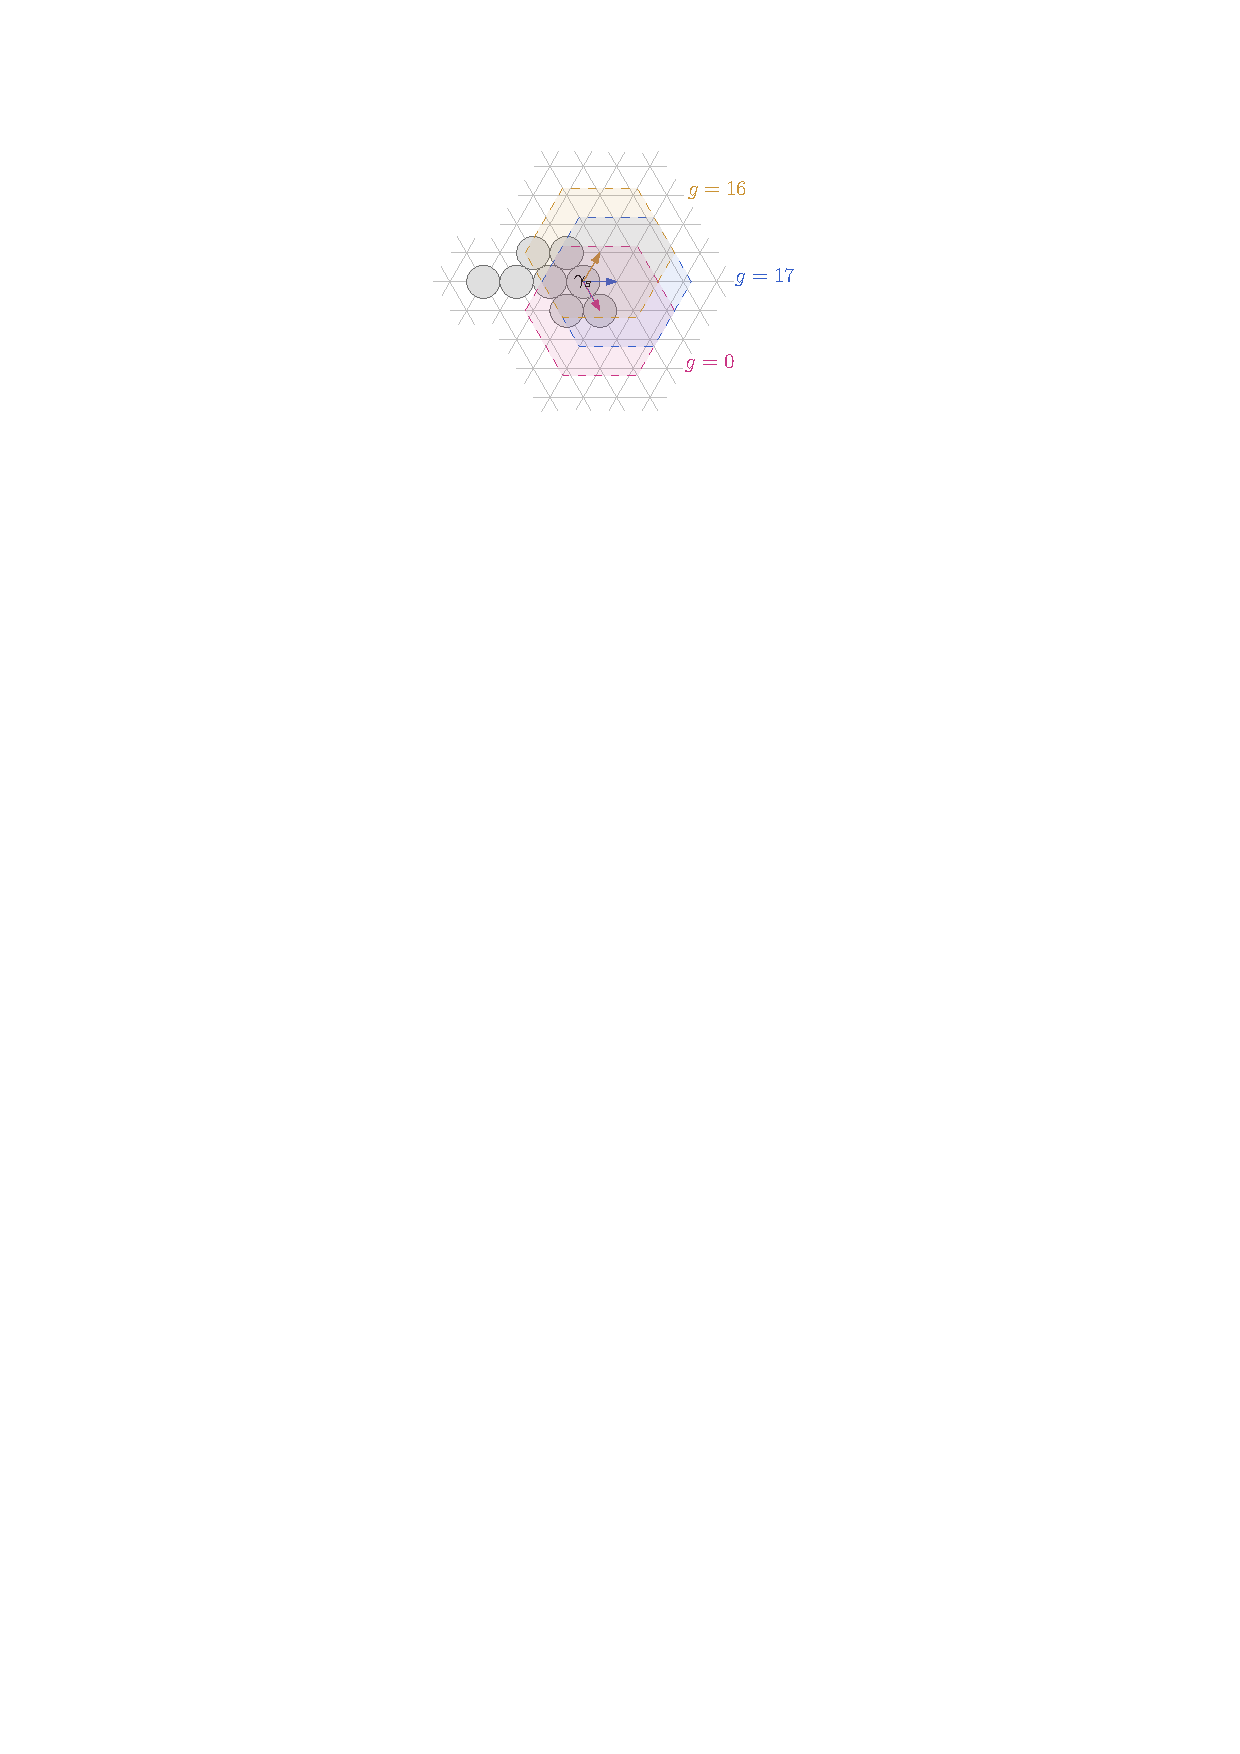
\includegraphics{graphics/ch5_principaldirection.pdf}
    \caption{The principal direction is chosen from one of three x-monotone options, here illustrated in different colors. The arrows represent the direction $\alpha$. The colored circles cover the two-step neighborhood $\Gamma^2(\coord_s + \alpha)$. From the previously assigned coordinates in $d_i$---the grey disks---within that area follows $g = g(\alpha)$.}
    \label{fig:ch5-principaldirection}
\end{figure}

The weight function $g$ evaluates a direction $\alpha$ as ``no space'' if it is not possible to embed the next spine vertex in direction $\alpha$ because the coordinate is immediately blocked.
Among the free two-step neighbors, it gives more weight to the immediately adjacent free coordinates, which are available for both branch and leaf disks, rather than those suitable only for leaves.

At the first step only, when there is no maximum embedded spine vertex, the principal direction is fixed to ``straight right'' without loss of generality.
The principal direction is evaluated only when embedding a spine vertex. The same principal direction then applies for embedding all adjacent branches and their leaves. Therefore, the direction which maximises the free space at index $i$ is the principal direction, i.e. 

\begin{equation*}
\alpha = \begin{cases}\underset{\alpha}{\arg \max}\, g(i, \alpha) & \text{ if $v_i \in \Spines$}\\
\underset{\alpha}{\arg \max}\, g(j-1, \alpha) & \text{ otherwise}
\end{cases}
\end{equation*}

Let $\coord^- = (x^-, y^-) = d_i(p(v_{i+1}))$ be the assigned x- and y-coordinates of the parent of the next vertex in order
\soeren{the next vertex in order. Also this order already has a name right? So the next vertex in $\leq_G$.}\peter{the ``next vertex in order'' is a term which I associated with $v_{i+1}$ above. I also added a clarification that $V$ is ordered earlier. should I still change it?}, and $\alpha = \overrightarrow e(\beta)$ the principal direction.

A coordinate $\coord = (x^- + x, y^- + y)$ is an \emph{upper coordinate} if $x \cdot \sin (-\beta) + y \cdot \cos (-\beta) > 0$. It is a \emph{lower coordinate} if $x \cdot \sin (-\beta) + y \cdot \cos (-\beta) < 0$.

The set $U = \{ \coord \in \Gamma^2(\coord^-) \mid \coord \text{ is an upper coordinate} \}$ is the \emph{upper area} and $L = \{ \coord \in \Gamma^2(\coord^-) \mid \coord \text{ is a lower coordinate} \}$ is the \emph{lower area}.

The \emph{affinity} $a \in \{-1, 1\}$ at step $i$ of the algorithm guides its decision for embedding of branches and leaves. It is defined as

\begin{equation*}
a = \begin{cases}1 & \text{ if } i = 0 \text{ or } f(i, L) \leq f(i, U), \\
-1 & \text{ otherwise.}
\end{cases}
\end{equation*}

\begin{figure}
    \centering
    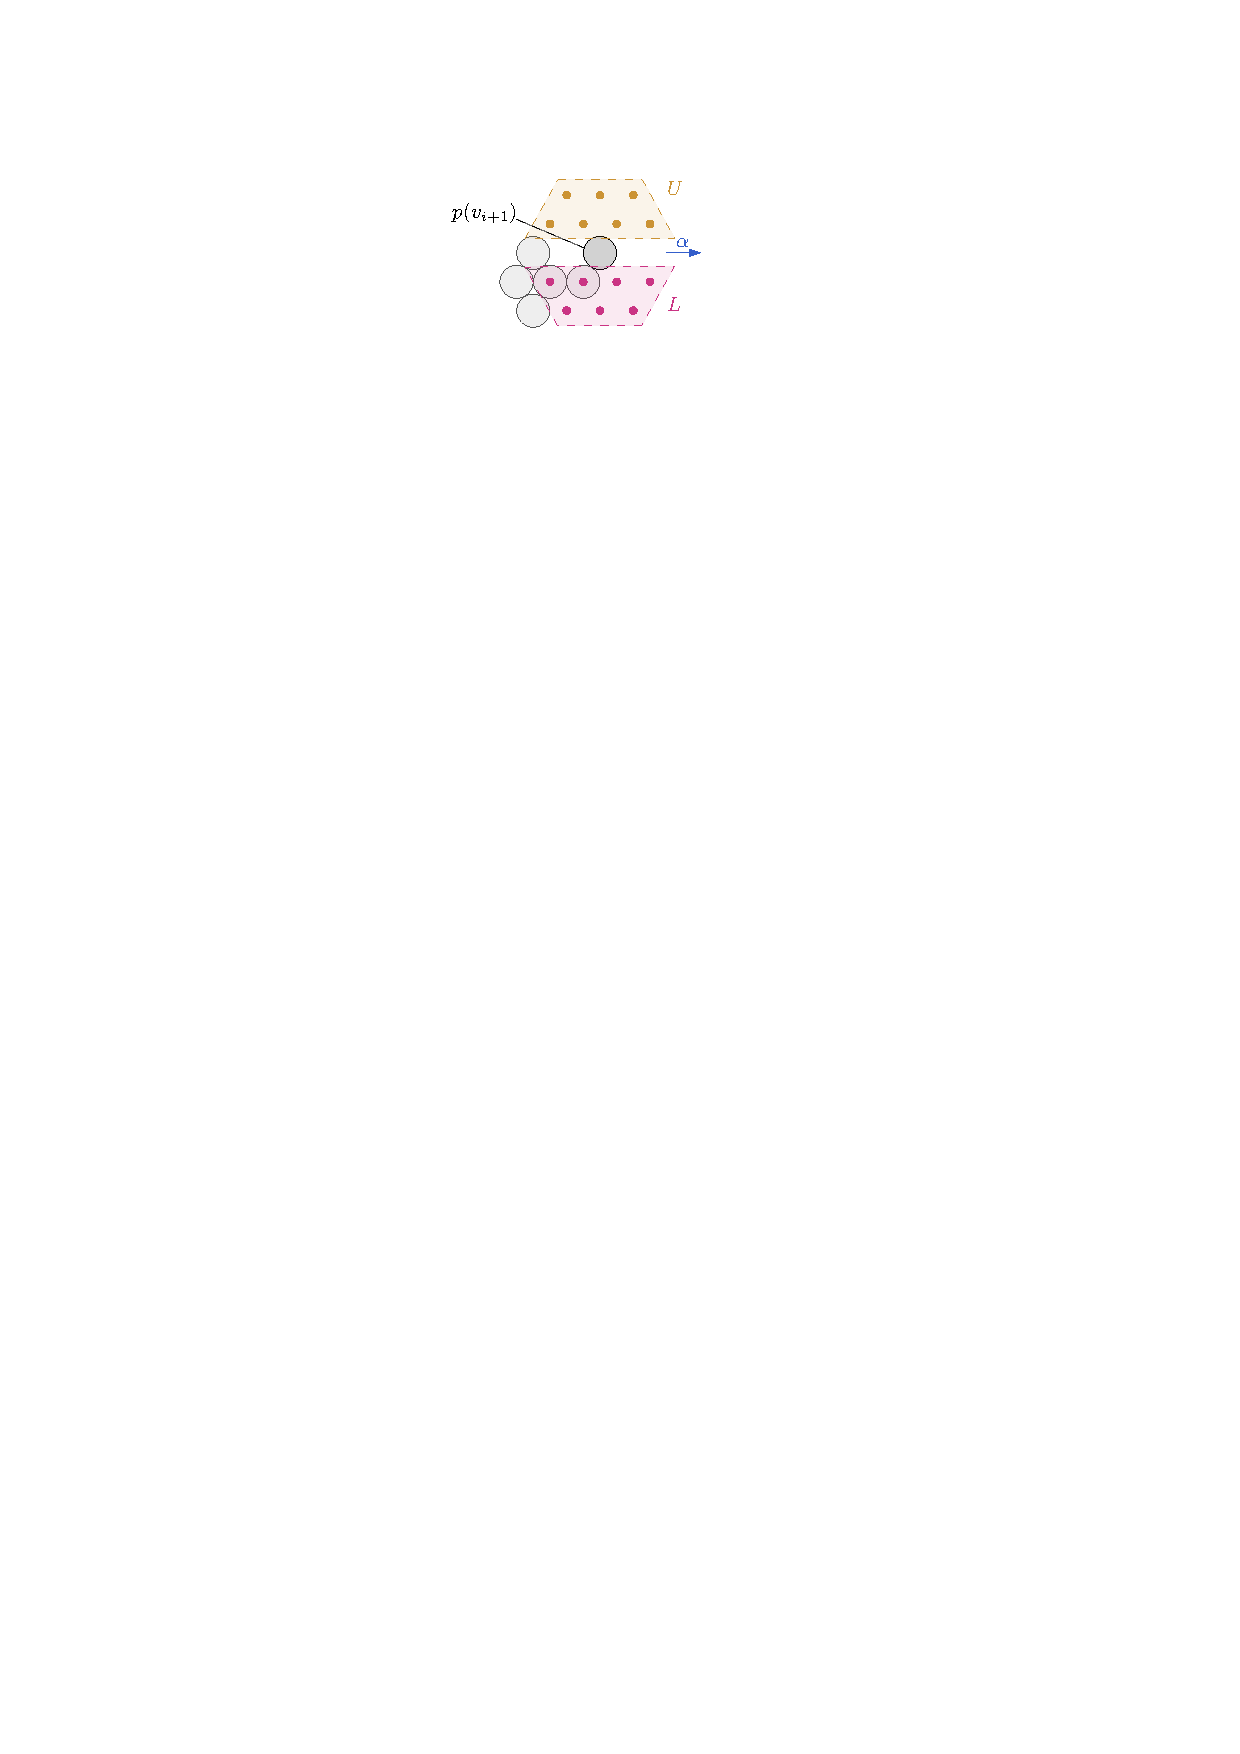
\includegraphics{graphics/ch5_affinity.pdf}
    \caption{The affinity biases the heuristic towards the upper or lower area, whichever contains more (weighted) free space. In this example, the coordinates marked by dots are part of the colored upper and lower area, which are determined from the position of the parent vertex disk in emphasized black and the principal direction $\alpha$.}
    \label{fig:ch5-affinity}
\end{figure}

Affinity compares available space ``above'' and ``below'' a line imagined through the parent coordinate $\coord^-$ along the principal direction. The heuristic thereby gains a tendency to embed a branch on the more spacious side of the spine, overall balancing disks on both sides. Coordinates on the side indicated by $a$ are preferred for assignment as described later in this chapter. Figure~\ref{fig:ch5-affinity} illustrates the concept.
\soeren[inline]{This definition is unclear to me. We should discuss what the goal is here and if this can be formulated in a different way. In any case, I think this definition would benefit from a figure.}\peter[inline]{clearer now?} Although our definition includes the special case of $i=0$, in which there is no parent vertex, this default has no bearing in practice because decisions on spine vertices are not affected by affinity.

We are now ready to formulate the criteria which apply in the selection of the $\texttt{heuristic}$ function output to determine our heuristic strategy.

\begin{enumerate}
    \item \emph{Bend heuristic}: when deciding the embedding coordinate for a spine vertex, we take a step in the principal direction from the previous spine vertex coordinate. This implements design goal~\ref{dg_bend}.
    \item \emph{Packing heuristic}: for branches and leaves, we prefer coordinates which lie further in the opposite of the principal direction. This implements design goal~\ref{dg_back}.
    \item \emph{Balance heuristic}: for branches and leaves, we strictly prefer coordinates matching the affinity. This implements design goal~\ref{dg_balance}.
    \item \emph{Space criterion}: coordinates with too few free neighboring coordinates to fit all the leaves are not valid branch candidates. This implements design goal~\ref{dg_space}.
\end{enumerate}

Among these decision criteria, higher precedence is given to higher number items. For branches and leaves in particular, the space criterion trumps balance, which trumps packing.

\begin{algorithm}
\SetKwFunction{Heuristic}{heuristic}
\SetKwFunction{PrincipalDirection}{principal\_direction}
\SetKwFunction{Affinity}{affinity}
\SetKw{Fail}{fail}
\SetKwData{G}{G}
\SetKwData{undef}{undef}
\SetKwData{Fundament}{F}
\SetKwProg{Fn}{Function}{}{}

\Fn{\Heuristic{$v_{i+1}, d_i$}}{
\KwIn{next vertex $v_{i+1}$, partial embedding function $d_i$}
\KwOut{embedding coordinate for $v_{i+1}$}
\KwData{lobster $G = (\Spines \cup \Branches \cup \Leaves, E)$, candidate coordinate $\kappa$}
$\coord_s \gets \max(v \in \Spines \wedge v \order v_{i+1})$\;
$\alpha \gets \PrincipalDirection(d_i, \coord_s)$\tcp*{bend heuristic}
\If{$v_{i+1} \in \Spines$}{
    \Return{$\coord_s + \alpha$}\;
}
$\coord_p \gets p(v_{i+1})$\;
$a \gets \Affinity(d_i, \coord_p, \alpha)$\tcp*{balance heuristic}
\For(\tcp*[f]{packing heuristic}){$\beta \text{ in } 180^\circ, 120^\circ, 60^\circ, 0^\circ, -60^\circ, -120^\circ$}{
    $\kappa \gets \coord_p + R(a \cdot \beta) \cdot \alpha$\;
    \If{$f(i, \kappa)$}{
        $\mathcal L \gets \{ l \in \Leaves \mid (v_i, l) \in E \}$\;
        \If(\tcp*[f]{space criterion}){$f(i, \Gamma(\kappa)) \geq |\mathcal L|$}{
            \Return{$\kappa$}\;
        }
    }
}
\Fail{}\tcp*{no representation found}

}
\caption{The heuristic decision function. We use the embedding order $\order$, the parent function $p$, the neighborhood function $\Gamma$ and the free space function $f$. The rotation matrix $R(\theta) = \begin{bmatrix}\cos \theta & -\sin \theta \\ \sin \theta & \cos \theta \end{bmatrix}$ helps us orient candidates relative to the principal direction $\alpha$.}
\label{alg:heuristic}
\end{algorithm}

The pseudocode in Algorithm~\ref{alg:heuristic} describes how the elements of the heuristic function come together. The spine bends in the principal direction, which promises the most free space. We evaluate candidate coordinates in back-to-front order to encourage tight packing. We distribute branches evenly above and below the spine by affinity, which tends to preserve the x-monotone spine coordinates as unassigned. We embed branches only where there is enough space left for leaves.

Consider this example involving precedence of the different considerations. If the next vertex is a branch and there is a ``far-back'' candidate coordinate at $\coord_s + \overrightarrow e(-120^\circ)$, when the affinity is $a=1$, the upper area candidate at $\coord_s + \overrightarrow e(60^\circ)$ is preferred. If there are 4 leaves on the branch and not enough free space in the neighborhood of the preferred candidate, $\coord_s + \overrightarrow e(0^\circ)$ is chosen instead, and so on until some candidate satisfies the space criterion.

\section{Breadth-First Order}
\label{section:ch5-bfs}

We also examine a variant of the heuristic algorithm that uses a different vertex embed order, denoted $\order^B$.

The original definition for $\order^D$ permits the case that, while embedding a particular subtree (branch and leaves), the algorithm might embed a leaf at a critical coordinate that would have been required as a free space for embedding some later branch vertex. Instead of embedding all the leaves on a branch directly after the branch vertex, the variant definition orders all branch vertices with the same parent spine to be embedded directly following that spine. Only then does it consider all the adjacent leaves.

We call this variant order the \emph{breadth-first} order to distinguish it from the previously defined depth-first order.

A breadth-first embedding order $\order^B$ is \emph{admissible} if it fulfills the following criteria, analogous to admissibility for a depth-first order.

\begin{itemize}
    \item $\order^B$ is a total order. It is reflexive, transitive and antisymmetric.
    \item $\order^B$ orders the spine like an admissible depth-first order.
    \item $\order^B$ groups branches and leaves together with their parent spine. 
     Let $s_1, s_2 \in \Spines, b \in \Branches, l \in \Leaves$ and $s_1 \order^B s_2$. If $s_1 = p(b)$, then $b \order^B s_2$. If $s_1 = p(p(l))$, then $l \order^B s_2$.
    \item $\order^B$ groups branches before leaves in a subtree. Let $s \in \Spines, b \in \Branches, l \in \Leaves, s = p(b)$ and $s = p(p(l))$. Then $b \order^B l$.
    \item Parent vertices come first. Let $v_1, v_2 \in V$. If $v_1 = p(v_2)$, then $v_1 \order^B v_2$.
\end{itemize}

Otherwise, the definition of the algorithm and heuristic function remain the same.


\chapter{Evaluation}

The two algorithms from Chapter~\ref{ch:dynprog} and Chapter~\ref{ch:heuristic} both decide Problem~\ref{prob:weak-udc-lobster} for size $n$ lobsters in time linear in $n$. In this chapter, we extend our understanding of their performance and correctness in practical application.

We provide a software implementation of the approaches. Then we measure the run time and answers on the exhaustively enumerated set of all lobster instances with spine length ranging from 2 to 7.

\section{Software Implementation}

Both algorithms are included in the functionality of the \texttt{udcrgen} (``unit disk contact representation generator'') program, which was entirely written as part of this thesis. \texttt{udcrgen} is written in C++ using the standard library and no other dependencies---though its unit tests do depend on Google Test~\cite{GoogleTest}. It uses the CMake~\cite{CMake} build system. The source code is available online.\footnote{\url{https://git.ac.tuwien.ac.at/soeren.nickel/peter_neubauer.git}}.

The program reads in a graph instance, runs one of the available algorithms on it and produces statistical output. This output contains, for every instance tested, the algorithm used, the instance size, spine count, recognition success (yes/no) and runtime. \soeren{What does statistical output mean here?}\peter{added details} If the instance is found to admit an embedding, \texttt{udcrgen} can also output such an embedding as a drawing.

It additionally offers ``benchmark mode'', in which it does not read an instance as input. Instead, it generates an enumeration of possible lobsters within user-specified restrictions on spine count given as input parameters. All generated instances become inputs for the algorithms. Though the enumeration omits some instances to save time, it covers enough to decide any lobster within the given limits. We describe the exact method in Section~\ref{section:ch6-enumeration} below. \soeren{What kind of equivalence? Maybe up to isomoprphism?}\peter{reformulated}

During execution, \texttt{udcrgen} produces diagnostic log messages at different levels of detail. The level and target log file can be configured by the user.

These algorithms are implemented in the program:

\begin{itemize}
    \item The ``strict contact'' algorithm described by Klemz et al.~\cite{Klemz2015}, with a configurable gap size for minimum distance of disks not in contact. It applies only to caterpillar graphs.
    \item The ``dynamic program'' described in Chapter~\ref{ch:dynprog}.
    \item The ``heuristic algorithm'' described in Chapter~\ref{ch:heuristic}. It features an ``embed order'' parameter, which selects either the depth-first or breadth-first order of vertices.
\end{itemize}

Input graphs may be given (if not generated) either

\begin{itemize}
    \item in a \emph{degree notation}---see Section~\ref{section:ch6-enumeration}---, which specifies the vertex degree of each spine vertex in a caterpillar, or
    \item as an \emph{edge list}, which may describe any graph. The program recognizes a caterpillar or lobster, if possible, and converts it to an internal representation as described in Section~\ref{section:ch6-graph-representation}. If provided with an unrecognized type of graph, the program terminates with an error.
\end{itemize}

The decision result and runtime measurement are recorded in a CSV file. The drawing(s) of yes-instances may be written to an \texttt{.ipe} file, the format of the IPE drawing editor~\cite{cheong_ipe_2022} (only in a single-instance mode), or in SVG format to an HTML file (also in benchmark mode).

\texttt{udcrgen} can also create an \emph{archive} consisting of two directories: one to hold all the yes-instances encountered, and another one for the no-instances. The archive uses a degree list format.

\section{Instance Enumeration}
\label{section:ch6-enumeration}

To exhaustively examine lobsters with $n$ spine vertices, we must define a systematic method of enumerating them. Our idea is based on the degree notation for lobsters. In this notation, a lobster with $n$ spine vertices is represented as an \emph{identifier} string $$d_{1,1}d_{1,2}d_{1,3}d_{1,4}d_{1,5}\_d_{2,1}d_{2,2}d_{2,3}d_{2,4}d_{2,5}\_\ldots\_d_{n,1}d_{n,2}d_{n,3}d_{n,4}d_{n,5},$$ where $d_{i,j} \in \{ \texttt x, 0, 1, 2, 3, 4, 5 \}$ is the number of leaf vertices adjacent to the $j$th branch on the $i$th spine vertex, or $\texttt x$ to signify ``no branch at this index''. We consider the $\texttt x$ equivalent to $-1$ for ordering purposes.
Any lobster instances with $n \geq 2$ that contain too many branches or leaves to be represented in this way certainly do not admit a disk contact embedding.\soeren[inline]{I'm not sure what the last sentence points out. Why is this specific to $n\leq 2$?}\peter[inline]{A single spine vertex is the only case that fits 6 branches. Should I add a comment to that effect?}

For all $1 \leq i \leq n, 1 \leq j \leq 5$ we initialize $d_{i,j} = \texttt x$, starting with a lobster consisting only of a spine without any branches. We instantiate the internal graph representation from the degree notation and test it with regards to the decision problem.
We obtain the next identifier by interpreting it like a $5n$-digit base-7 number, which we increment. If the last digit overflows, we carry the increment to the next digit and so on.

\begin{table}
\centering
\begin{tabular}{ r|r|r|r }
\toprule
Spine Length & Yes-Instances & No-Instances & Max. Vertex Count (Yes) \\
 \hline
2	 & 141	 	& 101 	& 24 \\
3	 & 1107	 	& 757 	& 29 \\
4	 & 9343	 	& 6297 	& 34 \\
5	 & 80952	& 54336 	& 39 \\
6	 & 698352	& 468667 	& 44 \\
7	 & 6041183	& 4053036 	& 49 \\
\bottomrule
\end{tabular}
 \caption{Through our enumeration, we discovered the listed number of lobsters. This enumeration is exhaustive for the given sizes, meaning that it accounts for every yes-instance for Problem~\ref{prob:weak-udc-lobster} up to efficient omissions by branch order, orientation and dominance discussed in this chapter. The no-instances are not exhaustive. They are simply informative about the arbitrary number of data points which emerged from our method of ``adding vertices until it fails''. This even lead us to evaluate lobsters with one more vertex than the ``maximum'', which naturally all fail quickly due to insufficient space. }
\label{tbl:instance-count}
\end{table}

By this naive method, the number of tests to run for size $n$ is $7^{5n}$. The actual number of instances which we evaluated in practice is listed in Table~\ref{tbl:instance-count}. We reduce the necessary work in several ways.

\subsection{Branch Ordering}

Since the minimum distance from a spine vertex is by definition the only distinguishing feature for any vertex in a lobster, we can always exchange any two branches of the same spine by swapping $d_{i,j}$ and $d_{i,k}$ in the representation. It still identifies the same lobster.
% We therefore define that $\texttt x < 0$
\soeren{For this purpose, you could define \texttt{x} as $-1$ in the thesis, even though the actual format is using \texttt{x}. This discrepancy can be specified in the definition.}\peter{done} We constrain our representation with the following \emph{branch ordering criterium}:

$$d_{i,j} \leq d_{i,k} \text{ if } j < k.$$

This reduces the valid representations to $\binom{7 + 5 - 1}{5}^n = 462^n,$ where $\binom{7 + 5 - 1}{5}$ is the number of 5-multisets from 7 elements.

\subsection{Orientation}

Let $s_1,\ldots,s_n$ be the sequence of spine sections---5 digits each. The sequence $s_n,\ldots,s_1$ then identifies the same lobster. We remove these duplicates from consideration by defining some arbitrary order $<_s$ over all valid spine constellations and enforce that the spine sequence must be \emph{canonically oriented}. A sequence has canonical orientation if

\begin{itemize}
    \item it is the empty sequence or
    \item $s_1 <_s s_n$ or
    \item $s_1 = s_n$ and $s_2, \ldots, s_{n-1}$ is canonically oriented.
\end{itemize}
%\soeren[inline]{Does this effectively half the number of considered sequences? Or can we make another statement about the effect on the number of considered instances.}
%\peter[inline]{Almost half (palindromes)}

\subsection{Dominance}

Let $$A = a_{1,1}a_{1,2}a_{1,3}a_{1,4}a_{1,5}\_\ldots\_a_{n,1}a_{n,2}a_{n,3}a_{n,4}a_{n,5}$$ and $$B = b_{1,1}b_{1,2}b_{1,3}b_{1,4}b_{1,5}\_\ldots\_b_{n,1}b_{n,2}b_{n,3}b_{n,4}b_{n,5}$$ be two lobster identifiers. Then $A$ \emph{dominates} $B$ if for all $1 \leq i \leq n, 1 \leq j \leq 5, a_{i,j} \leq b_{i,j}$. Since $A$ is easier than $B$, if we determine that $A$ does not admit an embedding, we infer that $B$ does not admit an embedding either and forgo testing the lobster described by $B$.

Similarly, if we would first determine that $B$ does admit an embedding, we may conclude that $A$ does as well. In practice, this does not help us because we examine our lobsters in strict incremental order.
%As an aside, note that this property might theoretically be exploited better by considering the set of spine constellations as a poset and locating the frontier of disk contact lobsters by binary search methods.
\soeren{Do you have a reference for binary search methods on posets?}\peter{No. Better drop the ``aside''.}

\subsection{Heuristic-Based Skip}

The test on any given lobster may, depending on the user's choice, involve running both the heuristic algorithm and the dynamic program. If this is the case, and if we are only interested in learning the answer to the decision problem (not in comparing the performance of the algorithms), then the fast heuristic solution should be attempted first. If it succeeds in finding that the input is a disk contact lobster, the slower exact algorithm can be skipped.

Our experiment, described below in Section~\ref{section:ch6-experiment}, does in fact compare algorithm performance. Thus we do not apply this particular optimization.

\section{Graph Representation}
\label{section:ch6-graph-representation}

The internal graph representation is the data structure which our algorithms operate on when they answer the disk contact problem. It must fulfill the following design criteria.

\begin{itemize}
    \item Sparsity---the structure should not store more than $O(n)$ data points for $n$ vertices.
    \item Fast traversal must be supported under admissible depth-first and breadth-first orders as defined in Chapter~\ref{ch:dynprog} and Chapter~\ref{ch:heuristic}.
    \item The query of relevant vertex properties must be fast:
    \begin{itemize}
        \item the depth of the vertex---0 for spines, 1 for branches and 2 for leaves and
        \item the number of children, i.e. vertices which have the queried vertex as their parent.
    \end{itemize}
    \item The internal representation must be easily convertible from the (user-supplied and generated) input graph formats as well as to the supported embedding output formats.
\end{itemize}

\begin{figure}
    \centering
    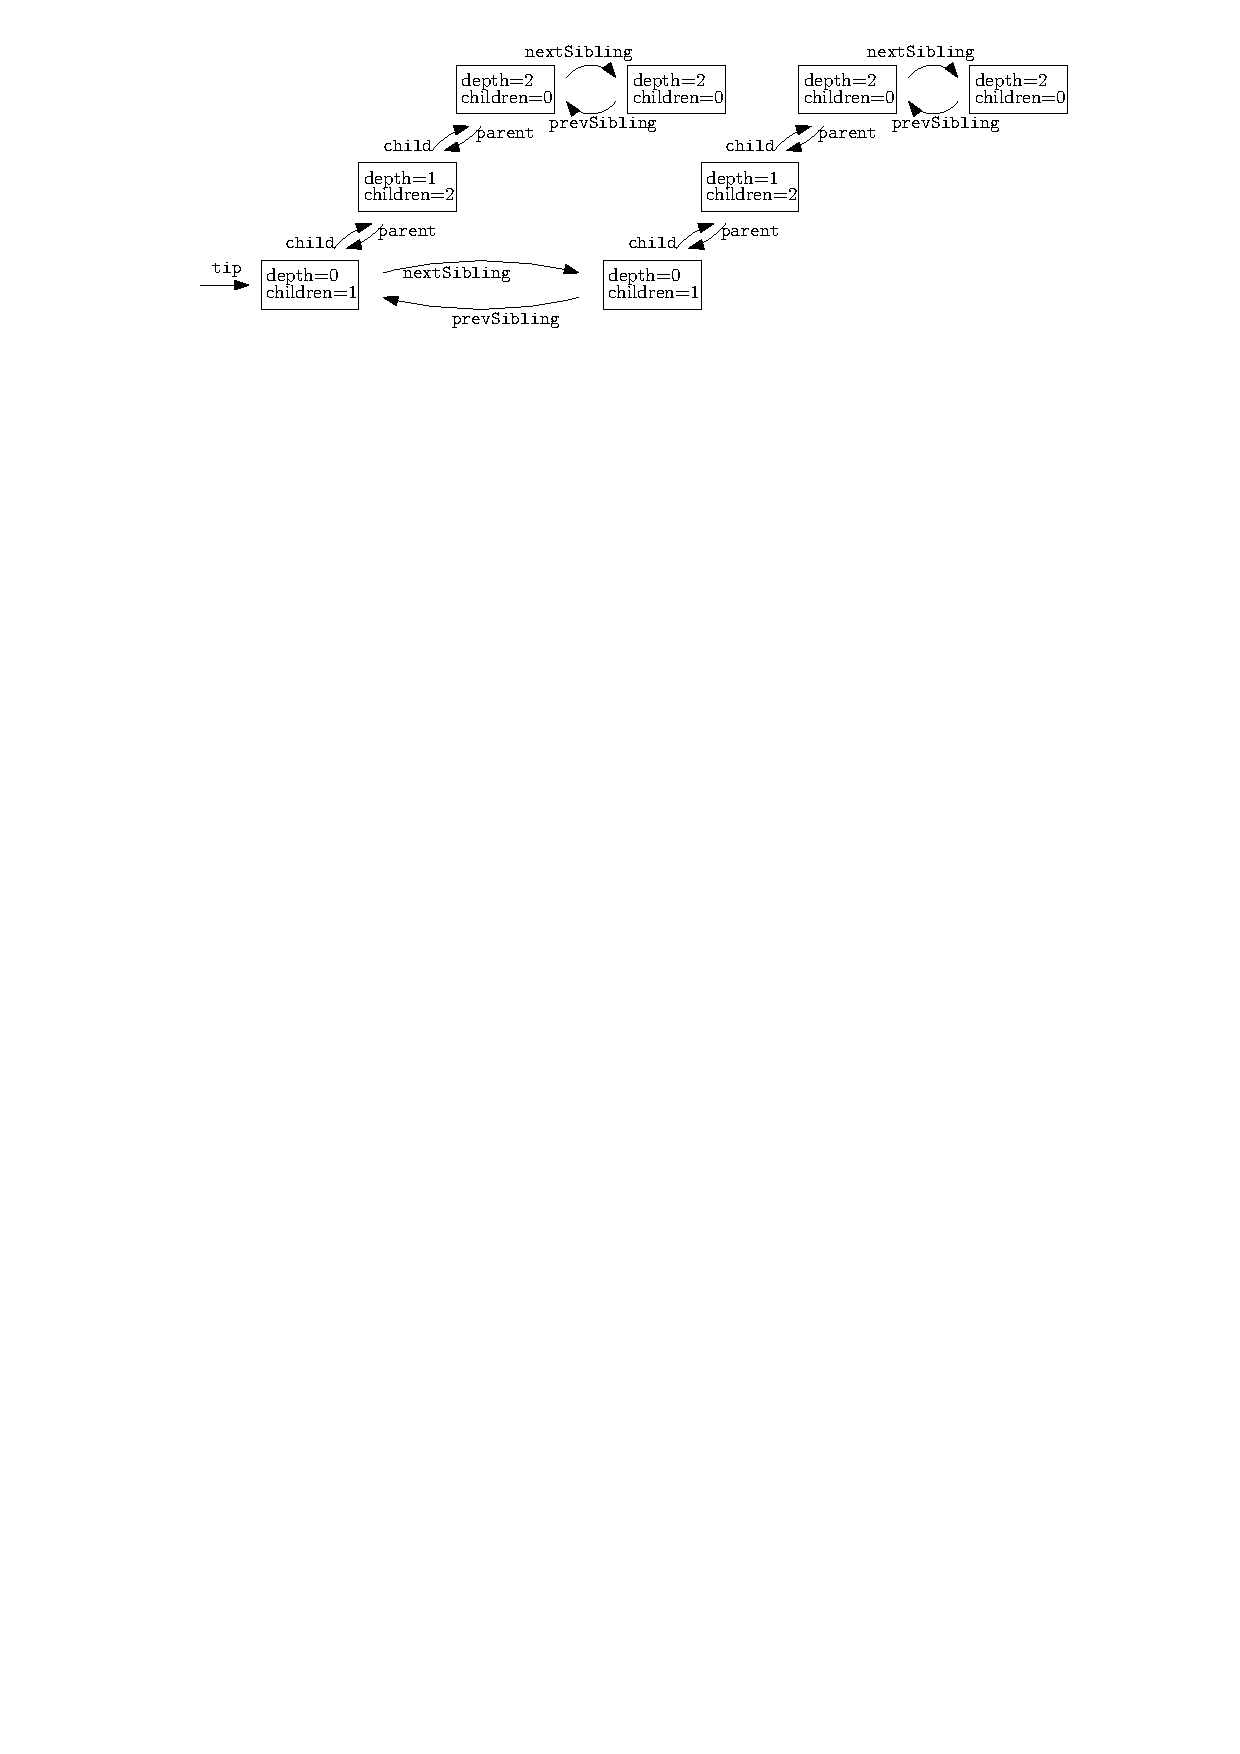
\includegraphics{graphics/ch6_diskgraph.pdf}
    \caption{The \texttt{DiskGraph} data structure with \texttt{Disk}s.}
    \label{fig:ch6_diskgraph}
\end{figure}

In the implementation, this structure is named \texttt{DiskGraph}. It holds a collection of \texttt{Disk}s and a pointer to the \texttt{tip}, which is the \texttt{Disk} that represents the first spine vertex. The \texttt{Disk} structure holds the vertex properties, including the constructed result of the (partial) embedding of that vertex. Figure~\ref{fig:ch6_diskgraph} illustrates the structure. \texttt{Disks} are represented by boxes and pointers by arrows.

\subsection{Format Conversion}

To convert from and to the degree list representations to the internal representation and also to produce the drawing from the coordinate data is trivial. However, the implementation can also accept an input graph as an edge list, which can describe any graph. In that case, we remove all the leaves to see if there remains just a string of vertices. If so, the graph is a caterpillar. Otherwise, we again remove all the leaves from the remainder to see if there remains just a string of vertices. If so, the graph is a lobster. We can reconstruct the removed graph components in reverse order.

These steps run in time $O(n)$ for $n$ input edges.
\soeren[inline]{I am not sure if we need this procedure in this detail. It kinda follows from the caterpillar definition. Let's discuss on Tuesday.}\peter[inline]{shortened}

\section{Experiment}
\label{section:ch6-experiment}

We ran the \texttt{udcrgen} software in benchmark mode with the dynamic programming algorithm, the heuristic algorithm with depth-first order and the heuristic algorithm with breadth-first order. The hardware specifications of the university-scale system used were: CPU: 2× Intel Xeon E5-2630 v2, 2.60GHz 6-core, RAM: 48GB.\soeren{This sentence is mssing something}\peter{better?} Note that the implementation is not parallelized.

The benchmark covers lobsters with at least $2$ and at most $7$ spine vertices enumerated using the scheme described in Section~\ref{section:ch6-enumeration}. In total, $11,414,272$ lobsters were evaluated.

\subsection{Dynamic Program Runtime}

\begin{figure}
    \centering % used for centering Figure
    \scalebox{1}{\includestandalone[]{standalone/runtime-dp}}
    \scalebox{1}{\includestandalone[]{standalone/runtime-dpyes}}
    \ref{legend:runtime-dp}
%     \centering
% \begin{tabular}{cc}
%     \includestandalone[]{standalone/runtime-dp} & \multirow{2}*{AAA\ref{legend:runtime-dp}} \\
%     \scalebox{1}{\includestandalone[]{standalone/runtime-dpyes}} & \\
% \end{tabular}
    \caption{The runtime of the dynamic program is depicted here. Every plotted point indicates the mean across all data points from the experiment with the same vertex count, spine length and instance class. Marks are colored and shaped according to the spine length and instance class. The second plot holds the same data, illustrating just the yes-instances.}
    \label{fig:ch5_runtime_dp}
\end{figure}

\begin{table}[t]
\centering
\begin{tabular}{ r|r|r|r|r|r|r }
\toprule
 $|V|$ & \#yes & \#no & $\varnothing \mu s$ DP/yes & $\varnothing \mu s$ DP/no & $\varnothing \mu s$ H/yes & $\varnothing \mu s$ H/no \\
 \hline
3	& 2 		& 0     	& 4.50		& 			& 6.50	&       \\
9	& 130		& 3     	& 30.55		& 80.75		& 18.49	& 15.50 \\
15	& 3272		& 385   	& 79.59		& 571.58	& 33.68	& 33.55 \\
21	& 31581		& 7028  	& 198.35	& 2,339.30	& 28.32	& 28.08 \\
27	& 151315	& 47442		& 396.52	& 4,428.87	& 39.14	& 38.48 \\
33	& 351093	& 157841	& 785.80	& 6,915.08	& 42.01	& 41.63 \\
39	& 402216	& 290471	& 1,414.34	& 9,979.08	& 51.02	& 49.88 \\
45	& 203481	& 251466	& 1,992.04	& 14,865.16	& 58.65	& 55.72 \\
\bottomrule
\end{tabular}
\caption{This excerpt of the experiment data shows the mean runtime of the dynamic program (under ``DP'') next to the heuristic with DFS order (under ``H''). The data is aggregated from all instances of the specified vertex count $|V|$ and class as specified in the header (``yes''/``no''). The number of data points aggregated in the ``DP'' columns is the same as the number of yes- and no-instances (``\#yes'', ``\#no'').}
\label{tbl:runtime}
\end{table}

In Figure~\ref{fig:ch5_runtime_dp} and Table~\ref{tbl:runtime}, we see the resulting average execution time of the dynamic program on lobsters of different sizes.

Among same-sized instances, those with a longer spine run faster. This is because there are fewer candidate coordinates for a spine vertex than for a branch vertex, and fewer candidates for a branch than a leaf.

We can observe that starting from about 25 vertices, the runtime of the dynamic programming algorithm is linear in the size of the input. The reason for the sharper rise in smaller instances, especially among yes-instances, is that the proportion of leaf vertices, which cause the greatest number of sub-problems to consider, grows initially and later remains constant in longer lobsters.

No-instances in our benchmark generally take far longer to compute than yes-instances. One reason is the early exit strategy discussed in Section~\ref{section:ch3_earlyexit}, which allows yes-instances to be answered without evaluating many of the generated sub-problems. Another reason is the way we enumerate instances, described above in Section~\ref{section:ch6-enumeration}. All our no-instances are at the brink of being ``almost solvable''. With these instances, we rarely encounter an early clog of too many vertices which would refute the instance. The algorithm is really forced to exhaust every possibility.

\subsection{Heuristic Runtime}

\begin{figure}[t]
    %\setlength{\unitlength}{0.14in} % selecting unit length
    \centering % used for centering Figure
    \scalebox{1}{\includestandalone[]{standalone/runtime-heuristic-dfs}}
    \scalebox{1}{\includestandalone[]{standalone/runtime-heuristic-bfs}}
    \ref{legend:runtime-heuristic}
    \caption{The runtime of the heuristic is depicted here both for depth-first and breadth-first order. Every plotted point indicates the mean across all data points from the experiment with the same vertex count, spine length and instance class. Marks are colored and shaped according to the spine length and instance class.}
    \label{fig:ch5_runtime_heuristic}
\end{figure}

\soeren[inline]{These figures are nice (although we need to change some things about the vertical axis labeling and maybe we can add a figure which puts the runtimes in relation to each other), but we need more explanation, both in the text and in the caption. Also we should discuss the consistent but discrete jumps at 19, 25, 32 and so on. Finally I think in particular to explain the jumps, the order in which things were ran on the cluster might actually be helpful here. Definitively we should discuss this on Tuesday.}

\begin{figure}
    %\setlength{\unitlength}{0.14in} % selecting unit length
    \centering % used for centering Figure
    \scalebox{1}{\includestandalone[]{standalone/runtime-dp-vs-h}}
    \caption{This is a direct comparison of the mean runtime of the dynamic program and the heuristic with DFS order. The scale is logarithmic, as at linear scale, the heuristic runtime simply appears flat at the bottom. Marks are colored and shaped by algorithm and instance class.}
    \label{fig:ch6-runtime-dp-vs-h}
\end{figure}
\peter[inline]{Neue Figure: Vergleich Heuristic vs Dynamic Prog (runtime)}

Figure~\ref{fig:ch5_runtime_heuristic} and Table~\ref{tbl:runtime} show the empirical runtime of the heuristic algorithm tested on the same set of instances as the dynamic program.

The same data in direct comparison with the dynamic program data is shown in Figure~\ref{fig:ch6-runtime-dp-vs-h}.

Overall, the heuristic offers up to about a $30\times$ speedup compared to the dynamic program on similar-sized yes-instances and about $250\times$ speedup compared to the dynamic program on our no-instances---which are, as mentioned before, generally unfavorable to the dynamic program.

While the dynamic program is faster on instances with more spines, the heuristic algorithm seems to require a small, fairly constant amount more time to place a spine in our implementation. The trend is linear in the vertex count of the instance, as expected. There is no performance difference between yes- and no-instances.

The consistent sudden increase in runtime around specific vertex counts, especially $15$ and $31$, are not related to any feature of the problem instances. Instead, they can probably be attributed to quirks of the \texttt{std::unordered\_map} associative data structure from the C++ standard library implementation used on the test system. This container holds the vertex coordinates in our heuristic algorithm implementation. The system used for the full experiment used GNU \texttt{libstdc++}, while the alternative experiment (on lobsters of spine length 2--4) depicted in Figure~\ref{fig:ch6-runtime-heuristic-alternative} ran on a Windows system using Microsoft's C++ standard library implementation. The alternative experiment does not show the same pattern of ``jumps''.

\begin{figure}
    %\setlength{\unitlength}{0.14in} % selecting unit length
    \centering % used for centering Figure
    \scalebox{1}{\includestandalone[]{standalone/runtime-heuristic-dfs-alternative}}
    \scalebox{1}{\includestandalone[]{standalone/runtime-heuristic-bfs-alternative}}
    \ref{legend:runtime-heuristic-alternative}
    \caption{The runtime of the heuristic as in Figure~\ref{fig:ch5_runtime_heuristic}, sampled on a different system for comparison.}
    \label{fig:ch6-runtime-heuristic-alternative}
\end{figure}

\subsection{Heuristic Accuracy}

\begin{figure}
    %\setlength{\unitlength}{0.14in} % selecting unit length
    \centering % used for centering Figure
    \scalebox{.8}{\includestandalone[]{standalone/accuracy}}
    \caption{The circles indicate the percentage of yes-instances correctly recognized by the two variations of the heuristic algorithm.}
    \label{fig:ch5_accuracy}
\end{figure}

\begin{table}
\centering
\begin{tabular}{ r|r|r|r|r }
\toprule
Spine Length & Yes-Instances & No-Instances & Yes (DFS) & Yes (BFS) \\
\hline
2	& 141	& 101			& 126	  (89\%) & 93      (66\%) \\
3	& 1107	& 757			& 1023	  (92\%) & 778     (70\%) \\
4	& 9343	& 6297			& 8092	  (87\%) & 6077    (65\%) \\
5	& 80952	& 54336			& 65635	  (81\%) & 48652   (60\%) \\
6	& 698352	& 468667	& 529979  (76\%) & 387235  (55\%) \\
7	& 6041183	& 4053036	& 4285811 (71\%) & 3090527 (51\%) \\
\bottomrule
\end{tabular}
\caption{Listing of the number of lobsters evaluated in the experiment, summed by spine length. The columns ``Yes (DFS)'' and ``Yes (BFS)'' show the absolute and relative number of lobsters which we know to be yes-instances (verified by the dynamic program) recognized as such by the heuristic using the indicated vertex order.}
\label{tbl:heuristic-accuracy}
\end{table}

Our heuristic approach with depth-first order answers between $70\%$--$90\%$ of all yes-instances of spine length 2--7 correctly. Figure~\ref{fig:ch5_accuracy} shows the percentages for the depth-first vertex order in red and compares it to the breadth-first variant in blue. The variant is shown to perform consistently worse by around $20$ percentage points.
\soeren[inline]{One final table giving the exact percentages and maybe the instance count would be nice here. Although we might want to include the instance count in the earlier suggested table.}



\chapter{Conclusion}

In this thesis, we reviewed the unit disk contact graph recognition problem and its complexity on different graph classes. We rigorously defined two main approaches to decide the tri-grid x-monotone weak UDC recognition problem on lobster graphs: the dynamic program as theorized by Bhore et al.~\cite{Bhore2021}, and a fast and less accurate heuristic approach as an original contribution.

The treatise on the dynamic program includes discussion on several strategies which improve performance. The heuristic is presented as two variants, which we compare in empirical evaluation. This evaluation shows that the depth-first variant is superior to the breadth-first variant.

We present \texttt{udcrgen}, a program that offers a software implementation of several different algorithms for UDC graph recognition: the recognition algorithm for caterpillars described by Klemz et al.~\cite{Klemz2015}, the dynamic program to recognize UDC lobsters as described in Chapter~\ref{ch:dynprog} and based on a proof by Bhore et al.~\cite{Bhore2021} and the original heuristic to recognize UDC lobsters as described in Chapter~\ref{ch:heuristic}. \texttt{udcrgen} supports a ``benchmark mode'' to exhaustively explore the space of small lobster instances with these algorithms and various input and output formats.

Our data from running the benchmark implementation demonstrates the real-world runtime that we can expect. It shows that the heuristic may yield a triple-digit speedup with accuracy declining from $90\%$ with increasing instance size in the answers.

\section{Open Questions}

Our results are specific to x-monotone representations on the triangular grid. Based on our lack of counter-examples, it might be reasonable to assume that these specific lobsters are the same that admit a weak UDC reprensention in general. Still, this assumption is so far unproven.

Imagine a counter-example which is not x-monotone. There is no intuitive way to define a UDC lobster in a way that will force the spine to ``bend back on itself''. The specimen would have to force this kind of constellation by tricky specification of branches and leaves, but will soon step on its own toes for lack of space around the spine. The embedded disks on both ends may only get in the way of each other.

Imagine another counter-example which is not restricted to the triangular grid. As discussed in Chapter~\ref{section:ch2-problems}, whether every lobster which admits a weak UDC also
admits a weak UDC on the triangular grid is an open question. Considering the small subtree depth of the lobster, the question is whether the difference between the tri-grid and some tighter packing can be relevant or even ruin the linear-time result.

The x-monotonicity concept can be described as a relaxation of an even tighter restriction, the \emph{straight spine}, in which no bends in the spine are allowed. Clearly, UDC lobsters do not all have a straight spine---a well-placed 4-leafed branch enforces a bend on a lobster that still admits an embedding perfectly fine. However, this leads us to consider whether x-monotonicity might be too relaxed. Perhaps it is sufficient to restrict UDC lobsters' spines to just two of the six cardinal directions of the triangular grid. We offer this conjecture as the final contribution of this thesis.

\begin{conjecture}[$60^\circ$-Monotone UDC Recognition for Lobsters]
Any lobster $G$ which admits a weak UDC representation also admits a weak UDC representation on the triangular grid wherein, for any two consecutive spine vertices $v$ and $u$, the angle between $\overrightarrow{vu}$ and the x-axis is either $0^\circ$ or $60^\circ$.
\end{conjecture}

We hope to have hereby contributed a small step towards further research on the much more significant open question:

\begin{displayquote}
What is a property $p(G)$, of any graph $G$, that holds if, and only if, the UDC problem for $G$ can be decided in linear time?
\end{displayquote}


\backmatter

% Use an optional list of figures.
% \listoffigures % Starred version, i.e., \listoffigures*, removes the toc entry.

% Use an optional list of tables.
% \cleardoublepage % Start list of tables on the next empty right hand page.
% \listoftables % Starred version, i.e., \listoftables*, removes the toc entry.

% Use an optional list of alogrithms.
% \listofalgorithms
% \addcontentsline{toc}{chapter}{List of Algorithms}

% Add an index.
% \printindex

% Add a glossary.
% \printglossaries

% Add a bibliography.
% \bibliographystyle{alpha}
% \bibliography{bsc_thesis}
\printbibliography

\end{document}